\chapter{Steiner Forest algorithms}

\section{Problem description}
Steiner Forest Problem (SFP)\\
Given an undirected graph $G = (V, E)$, a cost function on edges $c : E \rightarrow Q^+$, and a collection of disjoint subsets of $V$, $S_1, \dots S_k$, find a minimum cost subgraph in which each pair of vertices belonging to the same set $S_i$ is connected.
For $k = 1$ the problem is known as Steiner Tree Problem (STP).

\section{Primal-Dual Method algorithm}
Local searches written in our framework were compared to a 2-approximation algorithm described by Vazirani [Vazirani]. As far as we know, it's the best approximation algorithm for a SFP known to date.

Time complexity of provided implementation is $\Oh(S(E + V\alpha(V) + \log(S)))$ where $S = \sum_{i = 1}^{k}S_i$, $\alpha(V)$ is the inverse of the function $n = f(x) = A(x, x)$ and $A$ is Ackermann function.

\section{Create and break cycle local search}
Given some solution to Steiner Forest Problem ,,Create and break cycle'' (CBC) local search changes it by randomly adding edge between solution's vertices. If added edge created a cycle then the heaviest edge from this cycle is removed. It's obvious that obtained graph is still a feasible solution. After described operation it might happen that some edges are no longer needed like for example edges adjacent to leafs that don't belong to $S_i$ for any $i \in \{1, \dots k\}$. Therefore pruning procedure is used to ensure that only essential edges remains which might lead to further fitness improvement.

Provided Walker implementation takes $\Oh(V\log(V) + KV)$ time to prepare a step, where $K$ is a limit of attempts to choose a random edge with propierties as described above. In practice the limit is hardly ever reached and preparing step takes $\Oh(V\log(V)$.

\section{Minimum spanning tree of active vertices local search}
,,MST of active vertices'' (MSTAV) local search starts with some feasible solution of SFP. At each step a new solution is created by computing a pruned minimum spanning tree of $G'$ which is a subgraph of $G$ induced by some set of vertices $V'$ called active vertices. $V'$ is obtained from vertices belonging to the previous solution after randomly applying one of the following operations:
\begin{itemize}
\item add a random vertex that's not already in the set,
\item remove a random vertex from the set,
\item do both operations described above.
\end{itemize}

Note that it might happen that there is no feasible solution in $G'$. Therefore at the end of each step local search checks whether proposed solution is feasible and if it is not then it reverts any changes.

Provided Walker implementation takes $\Oh(E \log(V))$ time to prepare a step.

\section{Benchmarks}
To compare the algorithms we have used our randomly generated tests and a subset of SteinLib\footnote{\url{http://steinlib.zib.de}} tests for Steiner Tree Problem.
Names of tests generated by us can be expressed as regular expression $[s\ |\ d][E\ |\ R]V<\text{vertices count}>K<\text{terminal vertices count}>$. Letters $s, d$ tells whether graph is sparse or dense and letters $E, R$ tells accordingly whether graph is Euclidean or if edges were given random weight. Descriptions of SteinLib tests can be found at \url{http://steinlib.zib.de}.

In every test Walker starts with a pruned MST as starting solution.
\section{Results}

\subsection{Comparison of hill climbing and simulated annealing convergence}
TODO: krotko napisac, ze SA nie dziala i dlaczego ; dalej bede rozwazal tylko HillClimby

\begin{figure}[H]
\pgfsetplotmarksize{0pt}
\begin{figure}
 \centering
 \caption{\label{CBC-01dEV100K30}CBC-01dEV100K30},
 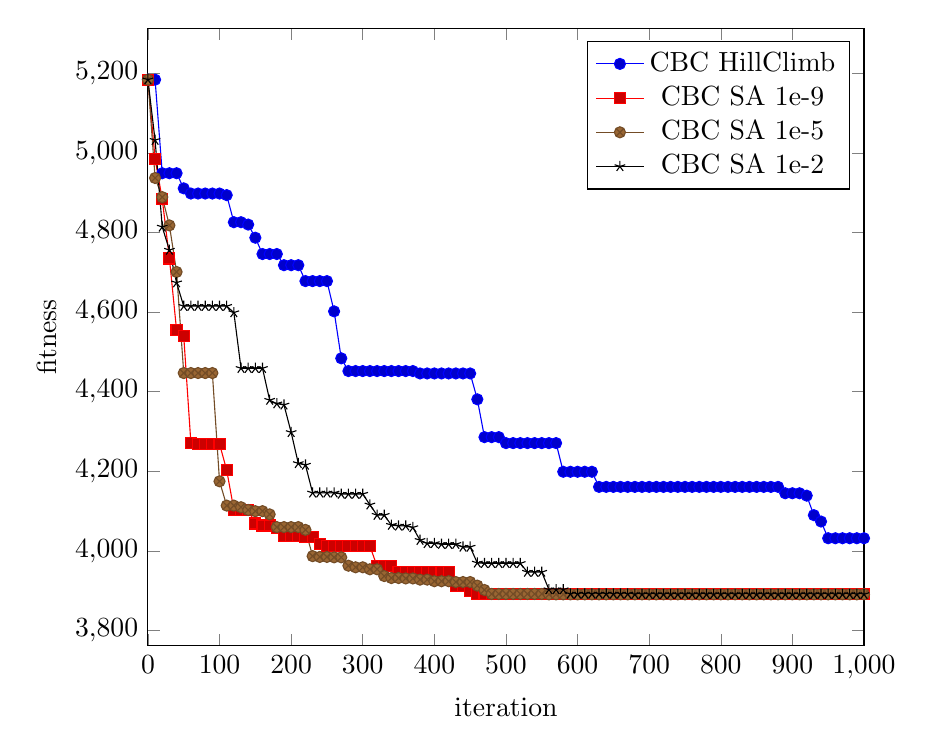
\begin{tikzpicture}
 \begin{axis}[
   width=0.75\textwidth,
   scale only axis,
   xlabel=iteration,
   ylabel=fitness,
   xmin=0,xmax=1000,
   domain=0:1000]
   \addplot coordinates {
     (0,5184)
     (10,5184)
     (20,4949)
     (30,4949)
     (40,4949)
     (50,4911)
     (60,4898)
     (70,4898)
     (80,4898)
     (90,4898)
     (100,4898)
     (110,4894)
     (120,4826)
     (130,4826)
     (140,4820)
     (150,4787)
     (160,4746)
     (170,4746)
     (180,4746)
     (190,4718)
     (200,4718)
     (210,4718)
     (220,4678)
     (230,4678)
     (240,4678)
     (250,4678)
     (260,4602)
     (270,4484)
     (280,4452)
     (290,4452)
     (300,4452)
     (310,4452)
     (320,4452)
     (330,4452)
     (340,4452)
     (350,4452)
     (360,4452)
     (370,4452)
     (380,4446)
     (390,4446)
     (400,4446)
     (410,4446)
     (420,4446)
     (430,4446)
     (440,4446)
     (450,4446)
     (460,4381)
     (470,4286)
     (480,4286)
     (490,4286)
     (500,4271)
     (510,4271)
     (520,4271)
     (530,4271)
     (540,4271)
     (550,4271)
     (560,4271)
     (570,4271)
     (580,4199)
     (590,4199)
     (600,4199)
     (610,4199)
     (620,4199)
     (630,4161)
     (640,4161)
     (650,4161)
     (660,4161)
     (670,4161)
     (680,4161)
     (690,4161)
     (700,4161)
     (710,4161)
     (720,4161)
     (730,4161)
     (740,4161)
     (750,4161)
     (760,4161)
     (770,4161)
     (780,4161)
     (790,4161)
     (800,4161)
     (810,4161)
     (820,4161)
     (830,4161)
     (840,4161)
     (850,4161)
     (860,4161)
     (870,4161)
     (880,4161)
     (890,4145)
     (900,4145)
     (910,4145)
     (920,4139)
     (930,4090)
     (940,4074)
     (950,4032)
     (960,4032)
     (970,4032)
     (980,4032)
     (990,4032)
     (1000,4032)
   };
   \addlegendentry{CBC HillClimb}
   \addplot coordinates {
     (0,5184)
     (10,4985)
     (20,4884)
     (30,4735)
     (40,4555)
     (50,4540)
     (60,4271)
     (70,4269)
     (80,4269)
     (90,4269)
     (100,4269)
     (110,4203)
     (120,4104)
     (130,4103)
     (140,4103)
     (150,4069)
     (160,4064)
     (170,4064)
     (180,4057)
     (190,4038)
     (200,4038)
     (210,4038)
     (220,4036)
     (230,4036)
     (240,4018)
     (250,4013)
     (260,4013)
     (270,4013)
     (280,4012)
     (290,4012)
     (300,4012)
     (310,4012)
     (320,3962)
     (330,3962)
     (340,3962)
     (350,3948)
     (360,3948)
     (370,3948)
     (380,3948)
     (390,3948)
     (400,3948)
     (410,3948)
     (420,3948)
     (430,3911)
     (440,3911)
     (450,3900)
     (460,3891)
     (470,3891)
     (480,3891)
     (490,3891)
     (500,3891)
     (510,3891)
     (520,3891)
     (530,3891)
     (540,3891)
     (550,3891)
     (560,3891)
     (570,3891)
     (580,3891)
     (590,3891)
     (600,3891)
     (610,3891)
     (620,3891)
     (630,3891)
     (640,3891)
     (650,3891)
     (660,3891)
     (670,3891)
     (680,3891)
     (690,3891)
     (700,3891)
     (710,3891)
     (720,3891)
     (730,3891)
     (740,3891)
     (750,3891)
     (760,3891)
     (770,3891)
     (780,3891)
     (790,3891)
     (800,3891)
     (810,3891)
     (820,3891)
     (830,3891)
     (840,3891)
     (850,3891)
     (860,3891)
     (870,3891)
     (880,3891)
     (890,3891)
     (900,3891)
     (910,3891)
     (920,3891)
     (930,3891)
     (940,3891)
     (950,3891)
     (960,3891)
     (970,3891)
     (980,3891)
     (990,3891)
     (1000,3891)
   };
   \addlegendentry{CBC SA 1e-9}
   \addplot coordinates {
     (0,5184)
     (10,4937)
     (20,4889)
     (30,4818)
     (40,4701)
     (50,4447)
     (60,4447)
     (70,4447)
     (80,4447)
     (90,4447)
     (100,4175)
     (110,4114)
     (120,4114)
     (130,4110)
     (140,4103)
     (150,4100)
     (160,4100)
     (170,4092)
     (180,4060)
     (190,4060)
     (200,4060)
     (210,4060)
     (220,4053)
     (230,3987)
     (240,3985)
     (250,3985)
     (260,3984)
     (270,3984)
     (280,3963)
     (290,3959)
     (300,3959)
     (310,3954)
     (320,3954)
     (330,3937)
     (340,3932)
     (350,3932)
     (360,3931)
     (370,3931)
     (380,3928)
     (390,3928)
     (400,3924)
     (410,3924)
     (420,3924)
     (430,3922)
     (440,3922)
     (450,3922)
     (460,3913)
     (470,3902)
     (480,3892)
     (490,3892)
     (500,3892)
     (510,3892)
     (520,3892)
     (530,3892)
     (540,3892)
     (550,3892)
     (560,3891)
     (570,3891)
     (580,3891)
     (590,3891)
     (600,3891)
     (610,3891)
     (620,3891)
     (630,3891)
     (640,3891)
     (650,3891)
     (660,3891)
     (670,3891)
     (680,3891)
     (690,3891)
     (700,3891)
     (710,3891)
     (720,3891)
     (730,3891)
     (740,3891)
     (750,3891)
     (760,3891)
     (770,3891)
     (780,3891)
     (790,3891)
     (800,3891)
     (810,3891)
     (820,3891)
     (830,3891)
     (840,3891)
     (850,3891)
     (860,3891)
     (870,3891)
     (880,3891)
     (890,3891)
     (900,3891)
     (910,3891)
     (920,3891)
     (930,3891)
     (940,3891)
     (950,3891)
     (960,3891)
     (970,3891)
     (980,3891)
     (990,3891)
     (1000,3891)
   };
   \addlegendentry{CBC SA 1e-5}
   \addplot coordinates {
     (0,5184)
     (10,5032)
     (20,4814)
     (30,4756)
     (40,4674)
     (50,4615)
     (60,4615)
     (70,4615)
     (80,4615)
     (90,4615)
     (100,4615)
     (110,4615)
     (120,4599)
     (130,4459)
     (140,4459)
     (150,4459)
     (160,4459)
     (170,4379)
     (180,4370)
     (190,4367)
     (200,4298)
     (210,4220)
     (220,4216)
     (230,4146)
     (240,4146)
     (250,4146)
     (260,4146)
     (270,4143)
     (280,4143)
     (290,4143)
     (300,4143)
     (310,4116)
     (320,4090)
     (330,4090)
     (340,4065)
     (350,4063)
     (360,4063)
     (370,4059)
     (380,4027)
     (390,4019)
     (400,4019)
     (410,4017)
     (420,4017)
     (430,4017)
     (440,4010)
     (450,4010)
     (460,3970)
     (470,3969)
     (480,3969)
     (490,3969)
     (500,3969)
     (510,3969)
     (520,3969)
     (530,3947)
     (540,3947)
     (550,3947)
     (560,3903)
     (570,3903)
     (580,3903)
     (590,3892)
     (600,3892)
     (610,3892)
     (620,3892)
     (630,3892)
     (640,3892)
     (650,3892)
     (660,3892)
     (670,3892)
     (680,3891)
     (690,3891)
     (700,3891)
     (710,3891)
     (720,3891)
     (730,3891)
     (740,3891)
     (750,3891)
     (760,3891)
     (770,3891)
     (780,3891)
     (790,3891)
     (800,3891)
     (810,3891)
     (820,3891)
     (830,3891)
     (840,3891)
     (850,3891)
     (860,3891)
     (870,3891)
     (880,3891)
     (890,3891)
     (900,3891)
     (910,3891)
     (920,3891)
     (930,3891)
     (940,3891)
     (950,3891)
     (960,3891)
     (970,3891)
     (980,3891)
     (990,3891)
     (1000,3891)
   };
   \addlegendentry{CBC SA 1e-2}
 \end{axis}
 \end{tikzpicture}
\end{figure}

\end{figure}
\begin{figure}[H]
\pgfsetplotmarksize{0pt}
\begin{figure}
 \centering
 \caption{\label{CBC-02dEV100K30}CBC-02dEV100K30},
 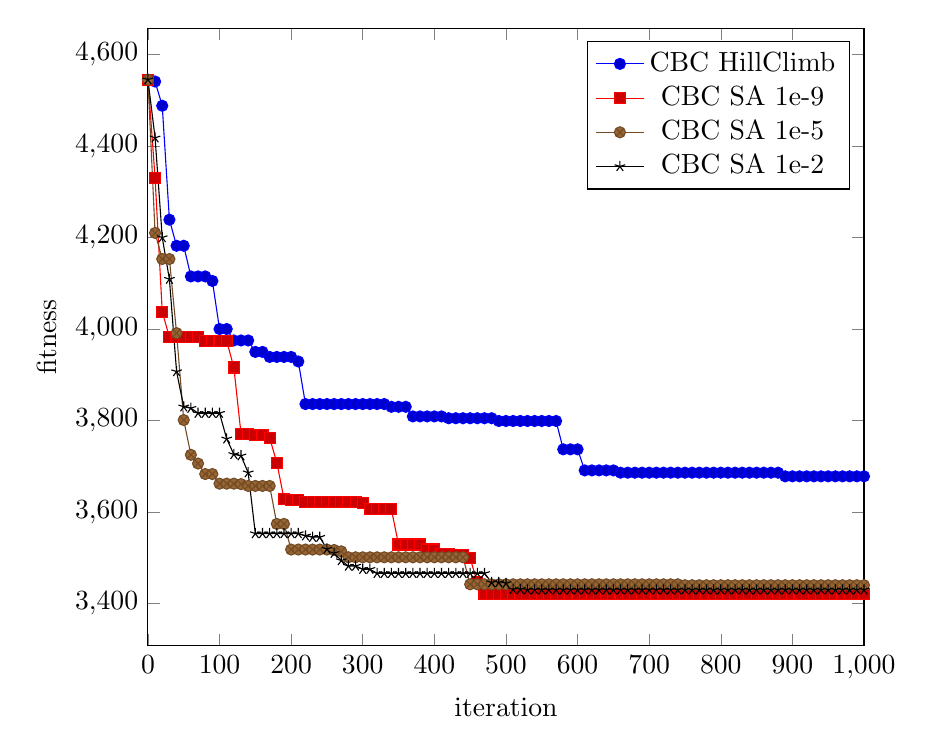
\begin{tikzpicture}
 \begin{axis}[
   width=0.75\textwidth,
   scale only axis,
   xlabel=iteration,
   ylabel=fitness,
   xmin=0,xmax=1000,
   domain=0:1000]
   \addplot coordinates {
     (0,4545)
     (10,4541)
     (20,4488)
     (30,4239)
     (40,4182)
     (50,4182)
     (60,4115)
     (70,4115)
     (80,4115)
     (90,4105)
     (100,4000)
     (110,4000)
     (120,3975)
     (130,3975)
     (140,3975)
     (150,3950)
     (160,3950)
     (170,3939)
     (180,3939)
     (190,3939)
     (200,3939)
     (210,3929)
     (220,3836)
     (230,3836)
     (240,3836)
     (250,3836)
     (260,3836)
     (270,3836)
     (280,3836)
     (290,3836)
     (300,3836)
     (310,3836)
     (320,3836)
     (330,3836)
     (340,3830)
     (350,3830)
     (360,3830)
     (370,3809)
     (380,3809)
     (390,3809)
     (400,3809)
     (410,3809)
     (420,3805)
     (430,3805)
     (440,3805)
     (450,3805)
     (460,3805)
     (470,3805)
     (480,3805)
     (490,3799)
     (500,3799)
     (510,3799)
     (520,3799)
     (530,3799)
     (540,3799)
     (550,3799)
     (560,3799)
     (570,3799)
     (580,3737)
     (590,3737)
     (600,3737)
     (610,3691)
     (620,3691)
     (630,3691)
     (640,3691)
     (650,3691)
     (660,3686)
     (670,3686)
     (680,3686)
     (690,3686)
     (700,3686)
     (710,3686)
     (720,3686)
     (730,3686)
     (740,3686)
     (750,3686)
     (760,3686)
     (770,3686)
     (780,3686)
     (790,3686)
     (800,3686)
     (810,3686)
     (820,3686)
     (830,3686)
     (840,3686)
     (850,3686)
     (860,3686)
     (870,3686)
     (880,3686)
     (890,3678)
     (900,3678)
     (910,3678)
     (920,3678)
     (930,3678)
     (940,3678)
     (950,3678)
     (960,3678)
     (970,3678)
     (980,3678)
     (990,3678)
     (1000,3678)
   };
   \addlegendentry{CBC HillClimb}
   \addplot coordinates {
     (0,4545)
     (10,4330)
     (20,4038)
     (30,3982)
     (40,3982)
     (50,3982)
     (60,3982)
     (70,3982)
     (80,3974)
     (90,3974)
     (100,3974)
     (110,3974)
     (120,3916)
     (130,3771)
     (140,3771)
     (150,3768)
     (160,3768)
     (170,3762)
     (180,3708)
     (190,3629)
     (200,3626)
     (210,3626)
     (220,3621)
     (230,3621)
     (240,3621)
     (250,3621)
     (260,3621)
     (270,3621)
     (280,3621)
     (290,3621)
     (300,3619)
     (310,3606)
     (320,3606)
     (330,3606)
     (340,3606)
     (350,3529)
     (360,3529)
     (370,3529)
     (380,3529)
     (390,3518)
     (400,3518)
     (410,3508)
     (420,3508)
     (430,3506)
     (440,3506)
     (450,3499)
     (460,3446)
     (470,3420)
     (480,3420)
     (490,3420)
     (500,3420)
     (510,3420)
     (520,3420)
     (530,3420)
     (540,3420)
     (550,3420)
     (560,3420)
     (570,3420)
     (580,3420)
     (590,3420)
     (600,3420)
     (610,3420)
     (620,3420)
     (630,3420)
     (640,3420)
     (650,3420)
     (660,3420)
     (670,3420)
     (680,3420)
     (690,3420)
     (700,3420)
     (710,3420)
     (720,3420)
     (730,3420)
     (740,3420)
     (750,3420)
     (760,3420)
     (770,3420)
     (780,3420)
     (790,3420)
     (800,3420)
     (810,3420)
     (820,3420)
     (830,3420)
     (840,3420)
     (850,3420)
     (860,3420)
     (870,3420)
     (880,3420)
     (890,3420)
     (900,3420)
     (910,3420)
     (920,3420)
     (930,3420)
     (940,3420)
     (950,3420)
     (960,3420)
     (970,3420)
     (980,3420)
     (990,3420)
     (1000,3420)
   };
   \addlegendentry{CBC SA 1e-9}
   \addplot coordinates {
     (0,4545)
     (10,4210)
     (20,4153)
     (30,4153)
     (40,3991)
     (50,3801)
     (60,3725)
     (70,3706)
     (80,3683)
     (90,3683)
     (100,3662)
     (110,3662)
     (120,3662)
     (130,3661)
     (140,3657)
     (150,3657)
     (160,3657)
     (170,3657)
     (180,3574)
     (190,3574)
     (200,3518)
     (210,3518)
     (220,3518)
     (230,3518)
     (240,3518)
     (250,3518)
     (260,3517)
     (270,3514)
     (280,3501)
     (290,3501)
     (300,3501)
     (310,3501)
     (320,3501)
     (330,3501)
     (340,3501)
     (350,3501)
     (360,3501)
     (370,3501)
     (380,3501)
     (390,3501)
     (400,3501)
     (410,3501)
     (420,3501)
     (430,3501)
     (440,3501)
     (450,3442)
     (460,3442)
     (470,3442)
     (480,3442)
     (490,3442)
     (500,3442)
     (510,3442)
     (520,3442)
     (530,3442)
     (540,3442)
     (550,3442)
     (560,3442)
     (570,3442)
     (580,3442)
     (590,3442)
     (600,3442)
     (610,3442)
     (620,3442)
     (630,3442)
     (640,3442)
     (650,3442)
     (660,3442)
     (670,3442)
     (680,3442)
     (690,3442)
     (700,3442)
     (710,3442)
     (720,3442)
     (730,3442)
     (740,3442)
     (750,3440)
     (760,3440)
     (770,3440)
     (780,3440)
     (790,3440)
     (800,3440)
     (810,3440)
     (820,3440)
     (830,3440)
     (840,3440)
     (850,3440)
     (860,3440)
     (870,3440)
     (880,3440)
     (890,3440)
     (900,3440)
     (910,3440)
     (920,3440)
     (930,3440)
     (940,3440)
     (950,3440)
     (960,3440)
     (970,3440)
     (980,3440)
     (990,3440)
     (1000,3440)
   };
   \addlegendentry{CBC SA 1e-5}
   \addplot coordinates {
     (0,4545)
     (10,4418)
     (20,4200)
     (30,4109)
     (40,3907)
     (50,3830)
     (60,3827)
     (70,3816)
     (80,3816)
     (90,3816)
     (100,3816)
     (110,3760)
     (120,3726)
     (130,3723)
     (140,3686)
     (150,3553)
     (160,3553)
     (170,3553)
     (180,3553)
     (190,3553)
     (200,3553)
     (210,3553)
     (220,3548)
     (230,3545)
     (240,3545)
     (250,3519)
     (260,3510)
     (270,3494)
     (280,3482)
     (290,3482)
     (300,3475)
     (310,3475)
     (320,3466)
     (330,3466)
     (340,3466)
     (350,3466)
     (360,3466)
     (370,3466)
     (380,3466)
     (390,3466)
     (400,3466)
     (410,3466)
     (420,3466)
     (430,3466)
     (440,3466)
     (450,3466)
     (460,3466)
     (470,3466)
     (480,3446)
     (490,3446)
     (500,3444)
     (510,3431)
     (520,3431)
     (530,3430)
     (540,3430)
     (550,3430)
     (560,3430)
     (570,3430)
     (580,3430)
     (590,3430)
     (600,3430)
     (610,3430)
     (620,3430)
     (630,3430)
     (640,3430)
     (650,3430)
     (660,3430)
     (670,3430)
     (680,3430)
     (690,3430)
     (700,3430)
     (710,3430)
     (720,3430)
     (730,3430)
     (740,3430)
     (750,3430)
     (760,3430)
     (770,3430)
     (780,3430)
     (790,3430)
     (800,3430)
     (810,3430)
     (820,3430)
     (830,3430)
     (840,3430)
     (850,3430)
     (860,3430)
     (870,3430)
     (880,3430)
     (890,3430)
     (900,3430)
     (910,3430)
     (920,3430)
     (930,3430)
     (940,3430)
     (950,3430)
     (960,3430)
     (970,3430)
     (980,3430)
     (990,3430)
     (1000,3430)
   };
   \addlegendentry{CBC SA 1e-2}
 \end{axis}
 \end{tikzpicture}
\end{figure}

\end{figure}
\begin{figure}[H]
\pgfsetplotmarksize{0pt}
\begin{figure}
 \centering
 \caption{\label{CBC-alue2087}CBC-alue2087},
 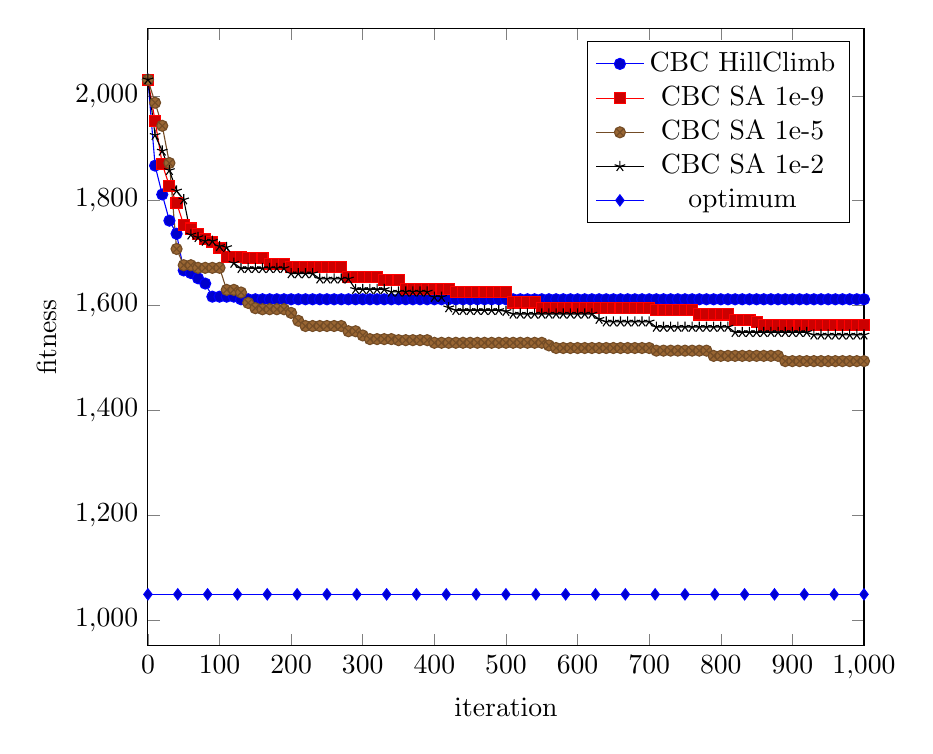
\begin{tikzpicture}
 \begin{axis}[
   width=0.75\textwidth,
   scale only axis,
   xlabel=iteration,
   ylabel=fitness,
   xmin=0,xmax=1000,
   domain=0:1000]
   \addplot coordinates {
     (0,2031)
     (10,1867)
     (20,1812)
     (30,1762)
     (40,1737)
     (50,1667)
     (60,1662)
     (70,1652)
     (80,1642)
     (90,1617)
     (100,1617)
     (110,1617)
     (120,1617)
     (130,1612)
     (140,1612)
     (150,1612)
     (160,1612)
     (170,1612)
     (180,1612)
     (190,1612)
     (200,1612)
     (210,1612)
     (220,1612)
     (230,1612)
     (240,1612)
     (250,1612)
     (260,1612)
     (270,1612)
     (280,1612)
     (290,1612)
     (300,1612)
     (310,1612)
     (320,1612)
     (330,1612)
     (340,1612)
     (350,1612)
     (360,1612)
     (370,1612)
     (380,1612)
     (390,1612)
     (400,1612)
     (410,1612)
     (420,1612)
     (430,1612)
     (440,1612)
     (450,1612)
     (460,1612)
     (470,1612)
     (480,1612)
     (490,1612)
     (500,1612)
     (510,1612)
     (520,1612)
     (530,1612)
     (540,1612)
     (550,1612)
     (560,1612)
     (570,1612)
     (580,1612)
     (590,1612)
     (600,1612)
     (610,1612)
     (620,1612)
     (630,1612)
     (640,1612)
     (650,1612)
     (660,1612)
     (670,1612)
     (680,1612)
     (690,1612)
     (700,1612)
     (710,1612)
     (720,1612)
     (730,1612)
     (740,1612)
     (750,1612)
     (760,1612)
     (770,1612)
     (780,1612)
     (790,1612)
     (800,1612)
     (810,1612)
     (820,1612)
     (830,1612)
     (840,1612)
     (850,1612)
     (860,1612)
     (870,1612)
     (880,1612)
     (890,1612)
     (900,1612)
     (910,1612)
     (920,1612)
     (930,1612)
     (940,1612)
     (950,1612)
     (960,1612)
     (970,1612)
     (980,1612)
     (990,1612)
     (1000,1612)
   };
   \addlegendentry{CBC HillClimb}
   \addplot coordinates {
     (0,2031)
     (10,1952)
     (20,1870)
     (30,1828)
     (40,1796)
     (50,1754)
     (60,1747)
     (70,1737)
     (80,1727)
     (90,1722)
     (100,1710)
     (110,1693)
     (120,1693)
     (130,1693)
     (140,1691)
     (150,1691)
     (160,1691)
     (170,1679)
     (180,1679)
     (190,1679)
     (200,1674)
     (210,1674)
     (220,1674)
     (230,1674)
     (240,1674)
     (250,1674)
     (260,1674)
     (270,1674)
     (280,1654)
     (290,1654)
     (300,1654)
     (310,1654)
     (320,1654)
     (330,1649)
     (340,1649)
     (350,1649)
     (360,1631)
     (370,1631)
     (380,1631)
     (390,1631)
     (400,1631)
     (410,1631)
     (420,1631)
     (430,1626)
     (440,1626)
     (450,1626)
     (460,1626)
     (470,1626)
     (480,1626)
     (490,1626)
     (500,1626)
     (510,1606)
     (520,1606)
     (530,1606)
     (540,1606)
     (550,1596)
     (560,1596)
     (570,1596)
     (580,1596)
     (590,1596)
     (600,1596)
     (610,1596)
     (620,1596)
     (630,1596)
     (640,1596)
     (650,1596)
     (660,1596)
     (670,1596)
     (680,1596)
     (690,1596)
     (700,1596)
     (710,1591)
     (720,1591)
     (730,1591)
     (740,1591)
     (750,1591)
     (760,1591)
     (770,1583)
     (780,1583)
     (790,1583)
     (800,1583)
     (810,1583)
     (820,1573)
     (830,1573)
     (840,1573)
     (850,1568)
     (860,1563)
     (870,1563)
     (880,1563)
     (890,1563)
     (900,1563)
     (910,1563)
     (920,1563)
     (930,1563)
     (940,1563)
     (950,1563)
     (960,1563)
     (970,1563)
     (980,1563)
     (990,1563)
     (1000,1563)
   };
   \addlegendentry{CBC SA 1e-9}
   \addplot coordinates {
     (0,2031)
     (10,1987)
     (20,1943)
     (30,1872)
     (40,1708)
     (50,1677)
     (60,1677)
     (70,1672)
     (80,1672)
     (90,1672)
     (100,1672)
     (110,1630)
     (120,1630)
     (130,1625)
     (140,1605)
     (150,1595)
     (160,1593)
     (170,1593)
     (180,1593)
     (190,1593)
     (200,1586)
     (210,1571)
     (220,1561)
     (230,1561)
     (240,1561)
     (250,1561)
     (260,1561)
     (270,1561)
     (280,1551)
     (290,1551)
     (300,1543)
     (310,1536)
     (320,1536)
     (330,1536)
     (340,1536)
     (350,1534)
     (360,1534)
     (370,1534)
     (380,1534)
     (390,1534)
     (400,1529)
     (410,1529)
     (420,1529)
     (430,1529)
     (440,1529)
     (450,1529)
     (460,1529)
     (470,1529)
     (480,1529)
     (490,1529)
     (500,1529)
     (510,1529)
     (520,1529)
     (530,1529)
     (540,1529)
     (550,1529)
     (560,1524)
     (570,1519)
     (580,1519)
     (590,1519)
     (600,1519)
     (610,1519)
     (620,1519)
     (630,1519)
     (640,1519)
     (650,1519)
     (660,1519)
     (670,1519)
     (680,1519)
     (690,1519)
     (700,1519)
     (710,1514)
     (720,1514)
     (730,1514)
     (740,1514)
     (750,1514)
     (760,1514)
     (770,1514)
     (780,1514)
     (790,1504)
     (800,1504)
     (810,1504)
     (820,1504)
     (830,1504)
     (840,1504)
     (850,1504)
     (860,1504)
     (870,1504)
     (880,1504)
     (890,1494)
     (900,1494)
     (910,1494)
     (920,1494)
     (930,1494)
     (940,1494)
     (950,1494)
     (960,1494)
     (970,1494)
     (980,1494)
     (990,1494)
     (1000,1494)
   };
   \addlegendentry{CBC SA 1e-5}
   \addplot coordinates {
     (0,2031)
     (10,1925)
     (20,1895)
     (30,1858)
     (40,1819)
     (50,1802)
     (60,1735)
     (70,1730)
     (80,1723)
     (90,1723)
     (100,1713)
     (110,1711)
     (120,1681)
     (130,1671)
     (140,1671)
     (150,1671)
     (160,1671)
     (170,1671)
     (180,1671)
     (190,1671)
     (200,1661)
     (210,1661)
     (220,1661)
     (230,1661)
     (240,1651)
     (250,1651)
     (260,1651)
     (270,1651)
     (280,1651)
     (290,1631)
     (300,1631)
     (310,1631)
     (320,1631)
     (330,1631)
     (340,1626)
     (350,1626)
     (360,1626)
     (370,1626)
     (380,1626)
     (390,1626)
     (400,1616)
     (410,1616)
     (420,1596)
     (430,1591)
     (440,1591)
     (450,1591)
     (460,1591)
     (470,1591)
     (480,1591)
     (490,1591)
     (500,1589)
     (510,1584)
     (520,1584)
     (530,1584)
     (540,1584)
     (550,1584)
     (560,1584)
     (570,1584)
     (580,1584)
     (590,1584)
     (600,1584)
     (610,1584)
     (620,1584)
     (630,1574)
     (640,1569)
     (650,1569)
     (660,1569)
     (670,1569)
     (680,1569)
     (690,1569)
     (700,1569)
     (710,1559)
     (720,1559)
     (730,1559)
     (740,1559)
     (750,1559)
     (760,1559)
     (770,1559)
     (780,1559)
     (790,1559)
     (800,1559)
     (810,1559)
     (820,1549)
     (830,1549)
     (840,1549)
     (850,1549)
     (860,1549)
     (870,1549)
     (880,1549)
     (890,1549)
     (900,1549)
     (910,1549)
     (920,1549)
     (930,1544)
     (940,1544)
     (950,1544)
     (960,1544)
     (970,1544)
     (980,1544)
     (990,1544)
     (1000,1544)
   };
   \addlegendentry{CBC SA 1e-2}
   \addplot {1049.000000};
   \addlegendentry{optimum}
 \end{axis}
 \end{tikzpicture}
\end{figure}

\end{figure}
\begin{figure}[H]
\pgfsetplotmarksize{0pt}
\begin{figure}
 \centering
 \caption{\label{CBC-berlin52}CBC-berlin52},
 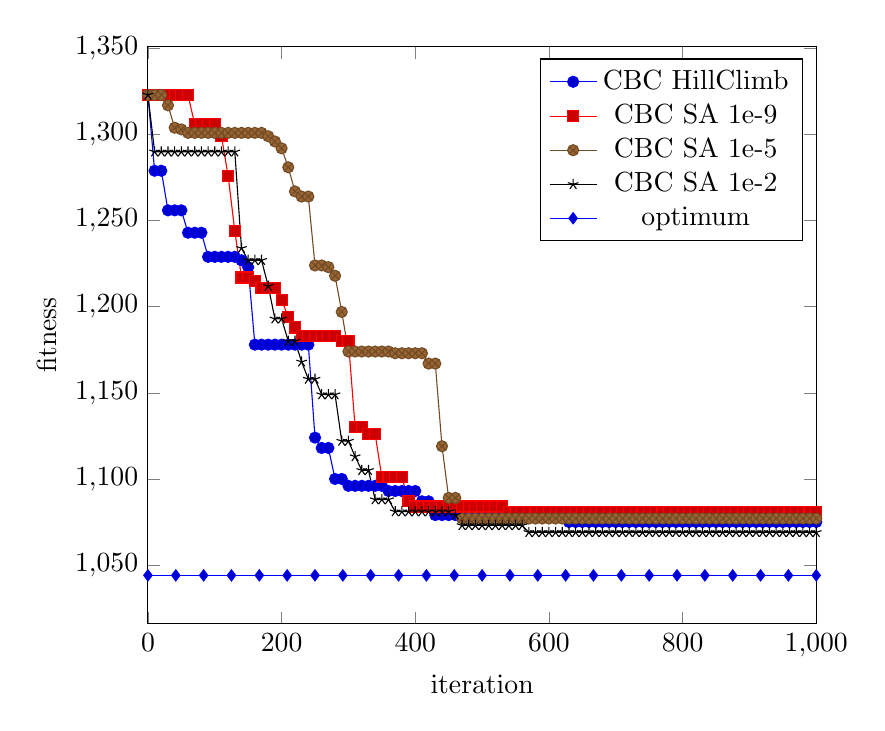
\begin{tikzpicture}
 \begin{axis}[
   width=0.7\textwidth,
   scale only axis,
   xlabel=iteration,
   ylabel=fitness,
   xmin=0,xmax=1000,
   domain=0:1000]
   \addplot coordinates {
     (0,1323)
     (10,1279)
     (20,1279)
     (30,1256)
     (40,1256)
     (50,1256)
     (60,1243)
     (70,1243)
     (80,1243)
     (90,1229)
     (100,1229)
     (110,1229)
     (120,1229)
     (130,1229)
     (140,1227)
     (150,1223)
     (160,1178)
     (170,1178)
     (180,1178)
     (190,1178)
     (200,1178)
     (210,1178)
     (220,1178)
     (230,1178)
     (240,1178)
     (250,1124)
     (260,1118)
     (270,1118)
     (280,1100)
     (290,1100)
     (300,1096)
     (310,1096)
     (320,1096)
     (330,1096)
     (340,1096)
     (350,1096)
     (360,1093)
     (370,1093)
     (380,1093)
     (390,1093)
     (400,1093)
     (410,1087)
     (420,1087)
     (430,1079)
     (440,1079)
     (450,1079)
     (460,1079)
     (470,1079)
     (480,1078)
     (490,1078)
     (500,1078)
     (510,1078)
     (520,1078)
     (530,1078)
     (540,1078)
     (550,1078)
     (560,1078)
     (570,1078)
     (580,1078)
     (590,1078)
     (600,1078)
     (610,1078)
     (620,1078)
     (630,1075)
     (640,1075)
     (650,1075)
     (660,1075)
     (670,1075)
     (680,1075)
     (690,1075)
     (700,1075)
     (710,1075)
     (720,1075)
     (730,1075)
     (740,1075)
     (750,1075)
     (760,1075)
     (770,1075)
     (780,1075)
     (790,1075)
     (800,1075)
     (810,1075)
     (820,1075)
     (830,1075)
     (840,1075)
     (850,1075)
     (860,1075)
     (870,1075)
     (880,1075)
     (890,1075)
     (900,1075)
     (910,1075)
     (920,1075)
     (930,1075)
     (940,1075)
     (950,1075)
     (960,1075)
     (970,1075)
     (980,1075)
     (990,1075)
     (1000,1075)
   };
   \addlegendentry{CBC HillClimb}
   \addplot coordinates {
     (0,1323)
     (10,1323)
     (20,1323)
     (30,1323)
     (40,1323)
     (50,1323)
     (60,1323)
     (70,1306)
     (80,1306)
     (90,1306)
     (100,1306)
     (110,1299)
     (120,1276)
     (130,1244)
     (140,1217)
     (150,1217)
     (160,1215)
     (170,1211)
     (180,1211)
     (190,1211)
     (200,1204)
     (210,1194)
     (220,1188)
     (230,1183)
     (240,1183)
     (250,1183)
     (260,1183)
     (270,1183)
     (280,1183)
     (290,1180)
     (300,1180)
     (310,1130)
     (320,1130)
     (330,1126)
     (340,1126)
     (350,1101)
     (360,1101)
     (370,1101)
     (380,1101)
     (390,1087)
     (400,1084)
     (410,1084)
     (420,1084)
     (430,1084)
     (440,1084)
     (450,1084)
     (460,1084)
     (470,1084)
     (480,1084)
     (490,1084)
     (500,1084)
     (510,1084)
     (520,1084)
     (530,1084)
     (540,1081)
     (550,1081)
     (560,1081)
     (570,1081)
     (580,1081)
     (590,1081)
     (600,1081)
     (610,1081)
     (620,1081)
     (630,1081)
     (640,1081)
     (650,1081)
     (660,1081)
     (670,1081)
     (680,1081)
     (690,1081)
     (700,1081)
     (710,1081)
     (720,1081)
     (730,1081)
     (740,1081)
     (750,1081)
     (760,1081)
     (770,1081)
     (780,1081)
     (790,1081)
     (800,1081)
     (810,1081)
     (820,1081)
     (830,1081)
     (840,1081)
     (850,1081)
     (860,1081)
     (870,1081)
     (880,1081)
     (890,1081)
     (900,1081)
     (910,1081)
     (920,1081)
     (930,1081)
     (940,1081)
     (950,1081)
     (960,1081)
     (970,1081)
     (980,1081)
     (990,1081)
     (1000,1081)
   };
   \addlegendentry{CBC SA 1e-9}
   \addplot coordinates {
     (0,1323)
     (10,1323)
     (20,1323)
     (30,1317)
     (40,1304)
     (50,1303)
     (60,1301)
     (70,1301)
     (80,1301)
     (90,1301)
     (100,1301)
     (110,1301)
     (120,1301)
     (130,1301)
     (140,1301)
     (150,1301)
     (160,1301)
     (170,1301)
     (180,1299)
     (190,1296)
     (200,1292)
     (210,1281)
     (220,1267)
     (230,1264)
     (240,1264)
     (250,1224)
     (260,1224)
     (270,1223)
     (280,1218)
     (290,1197)
     (300,1174)
     (310,1174)
     (320,1174)
     (330,1174)
     (340,1174)
     (350,1174)
     (360,1174)
     (370,1173)
     (380,1173)
     (390,1173)
     (400,1173)
     (410,1173)
     (420,1167)
     (430,1167)
     (440,1119)
     (450,1089)
     (460,1089)
     (470,1077)
     (480,1077)
     (490,1077)
     (500,1077)
     (510,1077)
     (520,1077)
     (530,1077)
     (540,1077)
     (550,1077)
     (560,1077)
     (570,1077)
     (580,1077)
     (590,1077)
     (600,1077)
     (610,1077)
     (620,1077)
     (630,1077)
     (640,1077)
     (650,1077)
     (660,1077)
     (670,1077)
     (680,1077)
     (690,1077)
     (700,1077)
     (710,1077)
     (720,1077)
     (730,1077)
     (740,1077)
     (750,1077)
     (760,1077)
     (770,1077)
     (780,1077)
     (790,1077)
     (800,1077)
     (810,1077)
     (820,1077)
     (830,1077)
     (840,1077)
     (850,1077)
     (860,1077)
     (870,1077)
     (880,1077)
     (890,1077)
     (900,1077)
     (910,1077)
     (920,1077)
     (930,1077)
     (940,1077)
     (950,1077)
     (960,1077)
     (970,1077)
     (980,1077)
     (990,1077)
     (1000,1077)
   };
   \addlegendentry{CBC SA 1e-5}
   \addplot coordinates {
     (0,1323)
     (10,1290)
     (20,1290)
     (30,1290)
     (40,1290)
     (50,1290)
     (60,1290)
     (70,1290)
     (80,1290)
     (90,1290)
     (100,1290)
     (110,1290)
     (120,1290)
     (130,1290)
     (140,1234)
     (150,1227)
     (160,1227)
     (170,1227)
     (180,1212)
     (190,1193)
     (200,1193)
     (210,1180)
     (220,1180)
     (230,1168)
     (240,1158)
     (250,1158)
     (260,1149)
     (270,1149)
     (280,1149)
     (290,1122)
     (300,1122)
     (310,1113)
     (320,1105)
     (330,1105)
     (340,1088)
     (350,1088)
     (360,1088)
     (370,1081)
     (380,1081)
     (390,1081)
     (400,1081)
     (410,1081)
     (420,1081)
     (430,1081)
     (440,1081)
     (450,1081)
     (460,1079)
     (470,1073)
     (480,1073)
     (490,1073)
     (500,1073)
     (510,1073)
     (520,1073)
     (530,1073)
     (540,1073)
     (550,1073)
     (560,1073)
     (570,1069)
     (580,1069)
     (590,1069)
     (600,1069)
     (610,1069)
     (620,1069)
     (630,1069)
     (640,1069)
     (650,1069)
     (660,1069)
     (670,1069)
     (680,1069)
     (690,1069)
     (700,1069)
     (710,1069)
     (720,1069)
     (730,1069)
     (740,1069)
     (750,1069)
     (760,1069)
     (770,1069)
     (780,1069)
     (790,1069)
     (800,1069)
     (810,1069)
     (820,1069)
     (830,1069)
     (840,1069)
     (850,1069)
     (860,1069)
     (870,1069)
     (880,1069)
     (890,1069)
     (900,1069)
     (910,1069)
     (920,1069)
     (930,1069)
     (940,1069)
     (950,1069)
     (960,1069)
     (970,1069)
     (980,1069)
     (990,1069)
     (1000,1069)
   };
   \addlegendentry{CBC SA 1e-2}
   \addplot {1044.000000};
   \addlegendentry{optimum}
 \end{axis}
 \end{tikzpicture}
\end{figure}

\end{figure}

\begin{figure}[H]
\pgfsetplotmarksize{0pt}
\begin{figure}
 \centering
 \caption{\label{MSTAV-01dEV100K30}MSTAV-01dEV100K30},
 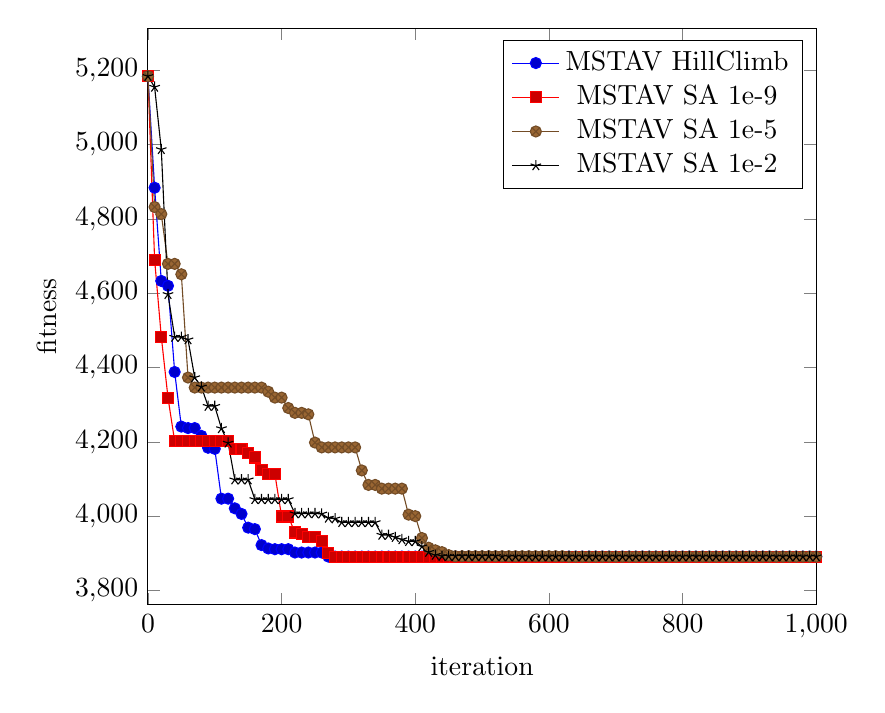
\begin{tikzpicture}
 \begin{axis}[
   width=0.7\textwidth,
   scale only axis,
   xlabel=iteration,
   ylabel=fitness,
   xmin=0,xmax=1000,
   domain=0:1000]
   \addplot coordinates {
     (0,5184)
     (10,4884)
     (20,4633)
     (30,4620)
     (40,4388)
     (50,4241)
     (60,4237)
     (70,4237)
     (80,4216)
     (90,4184)
     (100,4181)
     (110,4047)
     (120,4047)
     (130,4021)
     (140,4006)
     (150,3969)
     (160,3965)
     (170,3922)
     (180,3913)
     (190,3911)
     (200,3911)
     (210,3911)
     (220,3902)
     (230,3902)
     (240,3902)
     (250,3902)
     (260,3902)
     (270,3891)
     (280,3891)
     (290,3891)
     (300,3891)
     (310,3891)
     (320,3891)
     (330,3891)
     (340,3891)
     (350,3891)
     (360,3891)
     (370,3891)
     (380,3891)
     (390,3891)
     (400,3891)
     (410,3891)
     (420,3891)
     (430,3891)
     (440,3891)
     (450,3891)
     (460,3891)
     (470,3891)
     (480,3891)
     (490,3891)
     (500,3891)
     (510,3891)
     (520,3891)
     (530,3891)
     (540,3891)
     (550,3891)
     (560,3891)
     (570,3891)
     (580,3891)
     (590,3891)
     (600,3891)
     (610,3891)
     (620,3891)
     (630,3891)
     (640,3891)
     (650,3891)
     (660,3891)
     (670,3891)
     (680,3891)
     (690,3891)
     (700,3891)
     (710,3891)
     (720,3891)
     (730,3891)
     (740,3891)
     (750,3891)
     (760,3891)
     (770,3891)
     (780,3891)
     (790,3891)
     (800,3891)
     (810,3891)
     (820,3891)
     (830,3891)
     (840,3891)
     (850,3891)
     (860,3891)
     (870,3891)
     (880,3891)
     (890,3891)
     (900,3891)
     (910,3891)
     (920,3891)
     (930,3891)
     (940,3891)
     (950,3891)
     (960,3891)
     (970,3891)
     (980,3891)
     (990,3891)
     (1000,3891)
   };
   \addlegendentry{MSTAV HillClimb}
   \addplot coordinates {
     (0,5184)
     (10,4690)
     (20,4483)
     (30,4319)
     (40,4202)
     (50,4202)
     (60,4202)
     (70,4202)
     (80,4202)
     (90,4202)
     (100,4202)
     (110,4202)
     (120,4202)
     (130,4180)
     (140,4180)
     (150,4169)
     (160,4158)
     (170,4125)
     (180,4113)
     (190,4113)
     (200,3999)
     (210,3999)
     (220,3956)
     (230,3952)
     (240,3944)
     (250,3944)
     (260,3933)
     (270,3901)
     (280,3891)
     (290,3891)
     (300,3891)
     (310,3891)
     (320,3891)
     (330,3891)
     (340,3891)
     (350,3891)
     (360,3891)
     (370,3891)
     (380,3891)
     (390,3891)
     (400,3891)
     (410,3891)
     (420,3891)
     (430,3891)
     (440,3891)
     (450,3891)
     (460,3891)
     (470,3891)
     (480,3891)
     (490,3891)
     (500,3891)
     (510,3891)
     (520,3891)
     (530,3891)
     (540,3891)
     (550,3891)
     (560,3891)
     (570,3891)
     (580,3891)
     (590,3891)
     (600,3891)
     (610,3891)
     (620,3891)
     (630,3891)
     (640,3891)
     (650,3891)
     (660,3891)
     (670,3891)
     (680,3891)
     (690,3891)
     (700,3891)
     (710,3891)
     (720,3891)
     (730,3891)
     (740,3891)
     (750,3891)
     (760,3891)
     (770,3891)
     (780,3891)
     (790,3891)
     (800,3891)
     (810,3891)
     (820,3891)
     (830,3891)
     (840,3891)
     (850,3891)
     (860,3891)
     (870,3891)
     (880,3891)
     (890,3891)
     (900,3891)
     (910,3891)
     (920,3891)
     (930,3891)
     (940,3891)
     (950,3891)
     (960,3891)
     (970,3891)
     (980,3891)
     (990,3891)
     (1000,3891)
   };
   \addlegendentry{MSTAV SA 1e-9}
   \addplot coordinates {
     (0,5184)
     (10,4832)
     (20,4813)
     (30,4679)
     (40,4679)
     (50,4651)
     (60,4373)
     (70,4346)
     (80,4346)
     (90,4346)
     (100,4346)
     (110,4346)
     (120,4346)
     (130,4346)
     (140,4346)
     (150,4346)
     (160,4346)
     (170,4346)
     (180,4335)
     (190,4319)
     (200,4319)
     (210,4291)
     (220,4278)
     (230,4278)
     (240,4274)
     (250,4198)
     (260,4185)
     (270,4185)
     (280,4185)
     (290,4185)
     (300,4185)
     (310,4185)
     (320,4123)
     (330,4084)
     (340,4084)
     (350,4074)
     (360,4074)
     (370,4074)
     (380,4074)
     (390,4004)
     (400,4000)
     (410,3941)
     (420,3915)
     (430,3908)
     (440,3903)
     (450,3895)
     (460,3892)
     (470,3892)
     (480,3892)
     (490,3892)
     (500,3892)
     (510,3892)
     (520,3892)
     (530,3892)
     (540,3892)
     (550,3892)
     (560,3892)
     (570,3892)
     (580,3892)
     (590,3892)
     (600,3892)
     (610,3892)
     (620,3892)
     (630,3891)
     (640,3891)
     (650,3891)
     (660,3891)
     (670,3891)
     (680,3891)
     (690,3891)
     (700,3891)
     (710,3891)
     (720,3891)
     (730,3891)
     (740,3891)
     (750,3891)
     (760,3891)
     (770,3891)
     (780,3891)
     (790,3891)
     (800,3891)
     (810,3891)
     (820,3891)
     (830,3891)
     (840,3891)
     (850,3891)
     (860,3891)
     (870,3891)
     (880,3891)
     (890,3891)
     (900,3891)
     (910,3891)
     (920,3891)
     (930,3891)
     (940,3891)
     (950,3891)
     (960,3891)
     (970,3891)
     (980,3891)
     (990,3891)
     (1000,3891)
   };
   \addlegendentry{MSTAV SA 1e-5}
   \addplot coordinates {
     (0,5184)
     (10,5155)
     (20,4987)
     (30,4597)
     (40,4482)
     (50,4482)
     (60,4475)
     (70,4373)
     (80,4348)
     (90,4296)
     (100,4296)
     (110,4236)
     (120,4197)
     (130,4098)
     (140,4098)
     (150,4098)
     (160,4045)
     (170,4045)
     (180,4045)
     (190,4045)
     (200,4045)
     (210,4045)
     (220,4007)
     (230,4007)
     (240,4007)
     (250,4007)
     (260,4006)
     (270,3995)
     (280,3993)
     (290,3983)
     (300,3983)
     (310,3983)
     (320,3983)
     (330,3983)
     (340,3983)
     (350,3949)
     (360,3949)
     (370,3943)
     (380,3937)
     (390,3932)
     (400,3932)
     (410,3918)
     (420,3903)
     (430,3895)
     (440,3892)
     (450,3892)
     (460,3892)
     (470,3892)
     (480,3892)
     (490,3892)
     (500,3892)
     (510,3892)
     (520,3892)
     (530,3891)
     (540,3891)
     (550,3891)
     (560,3891)
     (570,3891)
     (580,3891)
     (590,3891)
     (600,3891)
     (610,3891)
     (620,3891)
     (630,3891)
     (640,3891)
     (650,3891)
     (660,3891)
     (670,3891)
     (680,3891)
     (690,3891)
     (700,3891)
     (710,3891)
     (720,3891)
     (730,3891)
     (740,3891)
     (750,3891)
     (760,3891)
     (770,3891)
     (780,3891)
     (790,3891)
     (800,3891)
     (810,3891)
     (820,3891)
     (830,3891)
     (840,3891)
     (850,3891)
     (860,3891)
     (870,3891)
     (880,3891)
     (890,3891)
     (900,3891)
     (910,3891)
     (920,3891)
     (930,3891)
     (940,3891)
     (950,3891)
     (960,3891)
     (970,3891)
     (980,3891)
     (990,3891)
     (1000,3891)
   };
   \addlegendentry{MSTAV SA 1e-2}
 \end{axis}
 \end{tikzpicture}
\end{figure}

\end{figure}
\begin{figure}[H]
\pgfsetplotmarksize{0pt}
\begin{figure}
 \centering
 \caption{\label{MSTAV-02dEV100K30}MSTAV-02dEV100K30},
 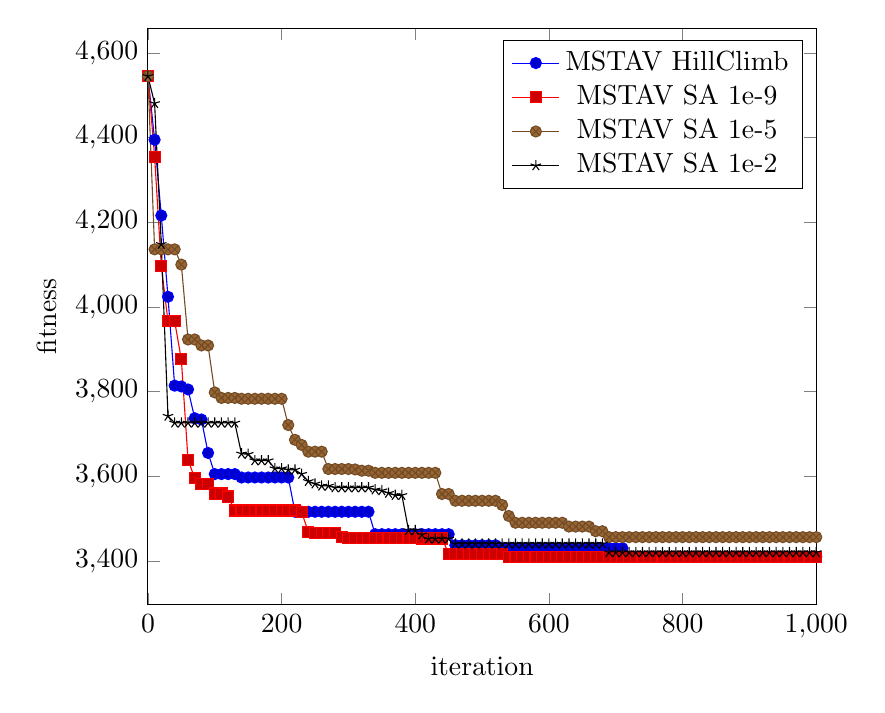
\begin{tikzpicture}
 \begin{axis}[
   width=0.7\textwidth,
   scale only axis,
   xlabel=iteration,
   ylabel=fitness,
   xmin=0,xmax=1000,
   domain=0:1000]
   \addplot coordinates {
     (0,4545)
     (10,4395)
     (20,4216)
     (30,4024)
     (40,3814)
     (50,3812)
     (60,3805)
     (70,3737)
     (80,3734)
     (90,3655)
     (100,3605)
     (110,3605)
     (120,3605)
     (130,3605)
     (140,3597)
     (150,3597)
     (160,3597)
     (170,3597)
     (180,3597)
     (190,3597)
     (200,3597)
     (210,3597)
     (220,3516)
     (230,3516)
     (240,3516)
     (250,3516)
     (260,3516)
     (270,3516)
     (280,3516)
     (290,3516)
     (300,3516)
     (310,3516)
     (320,3516)
     (330,3516)
     (340,3463)
     (350,3463)
     (360,3463)
     (370,3463)
     (380,3463)
     (390,3463)
     (400,3463)
     (410,3463)
     (420,3463)
     (430,3463)
     (440,3463)
     (450,3463)
     (460,3437)
     (470,3437)
     (480,3437)
     (490,3437)
     (500,3437)
     (510,3437)
     (520,3437)
     (530,3430)
     (540,3430)
     (550,3430)
     (560,3430)
     (570,3430)
     (580,3430)
     (590,3430)
     (600,3430)
     (610,3430)
     (620,3430)
     (630,3430)
     (640,3430)
     (650,3430)
     (660,3430)
     (670,3430)
     (680,3430)
     (690,3430)
     (700,3430)
     (710,3430)
     (720,3410)
     (730,3410)
     (740,3410)
     (750,3410)
     (760,3410)
     (770,3410)
     (780,3410)
     (790,3410)
     (800,3410)
     (810,3410)
     (820,3410)
     (830,3410)
     (840,3410)
     (850,3410)
     (860,3410)
     (870,3410)
     (880,3410)
     (890,3410)
     (900,3410)
     (910,3410)
     (920,3410)
     (930,3410)
     (940,3410)
     (950,3410)
     (960,3410)
     (970,3410)
     (980,3410)
     (990,3410)
     (1000,3410)
   };
   \addlegendentry{MSTAV HillClimb}
   \addplot coordinates {
     (0,4545)
     (10,4355)
     (20,4097)
     (30,3966)
     (40,3966)
     (50,3876)
     (60,3639)
     (70,3595)
     (80,3581)
     (90,3581)
     (100,3559)
     (110,3559)
     (120,3552)
     (130,3519)
     (140,3519)
     (150,3519)
     (160,3519)
     (170,3519)
     (180,3519)
     (190,3519)
     (200,3519)
     (210,3519)
     (220,3519)
     (230,3515)
     (240,3468)
     (250,3465)
     (260,3465)
     (270,3465)
     (280,3465)
     (290,3457)
     (300,3454)
     (310,3454)
     (320,3454)
     (330,3454)
     (340,3454)
     (350,3454)
     (360,3454)
     (370,3454)
     (380,3454)
     (390,3454)
     (400,3454)
     (410,3453)
     (420,3453)
     (430,3453)
     (440,3453)
     (450,3417)
     (460,3417)
     (470,3417)
     (480,3417)
     (490,3417)
     (500,3417)
     (510,3417)
     (520,3417)
     (530,3417)
     (540,3410)
     (550,3410)
     (560,3410)
     (570,3410)
     (580,3410)
     (590,3410)
     (600,3410)
     (610,3410)
     (620,3410)
     (630,3410)
     (640,3410)
     (650,3410)
     (660,3410)
     (670,3410)
     (680,3410)
     (690,3410)
     (700,3410)
     (710,3410)
     (720,3410)
     (730,3410)
     (740,3410)
     (750,3410)
     (760,3410)
     (770,3410)
     (780,3410)
     (790,3410)
     (800,3410)
     (810,3410)
     (820,3410)
     (830,3410)
     (840,3410)
     (850,3410)
     (860,3410)
     (870,3410)
     (880,3410)
     (890,3410)
     (900,3410)
     (910,3410)
     (920,3410)
     (930,3410)
     (940,3410)
     (950,3410)
     (960,3410)
     (970,3410)
     (980,3410)
     (990,3410)
     (1000,3410)
   };
   \addlegendentry{MSTAV SA 1e-9}
   \addplot coordinates {
     (0,4545)
     (10,4136)
     (20,4136)
     (30,4136)
     (40,4136)
     (50,4100)
     (60,3923)
     (70,3923)
     (80,3909)
     (90,3909)
     (100,3798)
     (110,3785)
     (120,3785)
     (130,3785)
     (140,3783)
     (150,3783)
     (160,3783)
     (170,3783)
     (180,3783)
     (190,3783)
     (200,3783)
     (210,3721)
     (220,3686)
     (230,3674)
     (240,3658)
     (250,3658)
     (260,3658)
     (270,3617)
     (280,3617)
     (290,3617)
     (300,3617)
     (310,3616)
     (320,3613)
     (330,3613)
     (340,3608)
     (350,3608)
     (360,3608)
     (370,3608)
     (380,3608)
     (390,3608)
     (400,3608)
     (410,3608)
     (420,3608)
     (430,3608)
     (440,3558)
     (450,3558)
     (460,3542)
     (470,3542)
     (480,3542)
     (490,3542)
     (500,3542)
     (510,3542)
     (520,3542)
     (530,3532)
     (540,3506)
     (550,3490)
     (560,3490)
     (570,3490)
     (580,3490)
     (590,3490)
     (600,3490)
     (610,3490)
     (620,3490)
     (630,3481)
     (640,3481)
     (650,3481)
     (660,3481)
     (670,3470)
     (680,3470)
     (690,3456)
     (700,3456)
     (710,3456)
     (720,3456)
     (730,3456)
     (740,3456)
     (750,3456)
     (760,3456)
     (770,3456)
     (780,3456)
     (790,3456)
     (800,3456)
     (810,3456)
     (820,3456)
     (830,3456)
     (840,3456)
     (850,3456)
     (860,3456)
     (870,3456)
     (880,3456)
     (890,3456)
     (900,3456)
     (910,3456)
     (920,3456)
     (930,3456)
     (940,3456)
     (950,3456)
     (960,3456)
     (970,3456)
     (980,3456)
     (990,3456)
     (1000,3456)
   };
   \addlegendentry{MSTAV SA 1e-5}
   \addplot coordinates {
     (0,4545)
     (10,4481)
     (20,4148)
     (30,3742)
     (40,3726)
     (50,3726)
     (60,3726)
     (70,3726)
     (80,3726)
     (90,3726)
     (100,3726)
     (110,3726)
     (120,3726)
     (130,3726)
     (140,3653)
     (150,3652)
     (160,3637)
     (170,3637)
     (180,3637)
     (190,3618)
     (200,3618)
     (210,3615)
     (220,3615)
     (230,3605)
     (240,3588)
     (250,3582)
     (260,3577)
     (270,3577)
     (280,3573)
     (290,3573)
     (300,3573)
     (310,3573)
     (320,3573)
     (330,3573)
     (340,3568)
     (350,3566)
     (360,3560)
     (370,3555)
     (380,3555)
     (390,3472)
     (400,3472)
     (410,3462)
     (420,3452)
     (430,3452)
     (440,3452)
     (450,3452)
     (460,3440)
     (470,3440)
     (480,3440)
     (490,3440)
     (500,3440)
     (510,3440)
     (520,3440)
     (530,3440)
     (540,3440)
     (550,3440)
     (560,3440)
     (570,3440)
     (580,3440)
     (590,3440)
     (600,3440)
     (610,3440)
     (620,3440)
     (630,3440)
     (640,3440)
     (650,3440)
     (660,3440)
     (670,3440)
     (680,3440)
     (690,3420)
     (700,3420)
     (710,3420)
     (720,3420)
     (730,3420)
     (740,3420)
     (750,3420)
     (760,3420)
     (770,3420)
     (780,3420)
     (790,3420)
     (800,3420)
     (810,3420)
     (820,3420)
     (830,3420)
     (840,3420)
     (850,3420)
     (860,3420)
     (870,3420)
     (880,3420)
     (890,3420)
     (900,3420)
     (910,3420)
     (920,3420)
     (930,3420)
     (940,3420)
     (950,3420)
     (960,3420)
     (970,3420)
     (980,3420)
     (990,3420)
     (1000,3420)
   };
   \addlegendentry{MSTAV SA 1e-2}
 \end{axis}
 \end{tikzpicture}
\end{figure}

\end{figure}
\begin{figure}[H]
\pgfsetplotmarksize{0pt}
 \centering
 \caption{\label{MSTAV-alue2087}MSTAV-alue2087},
 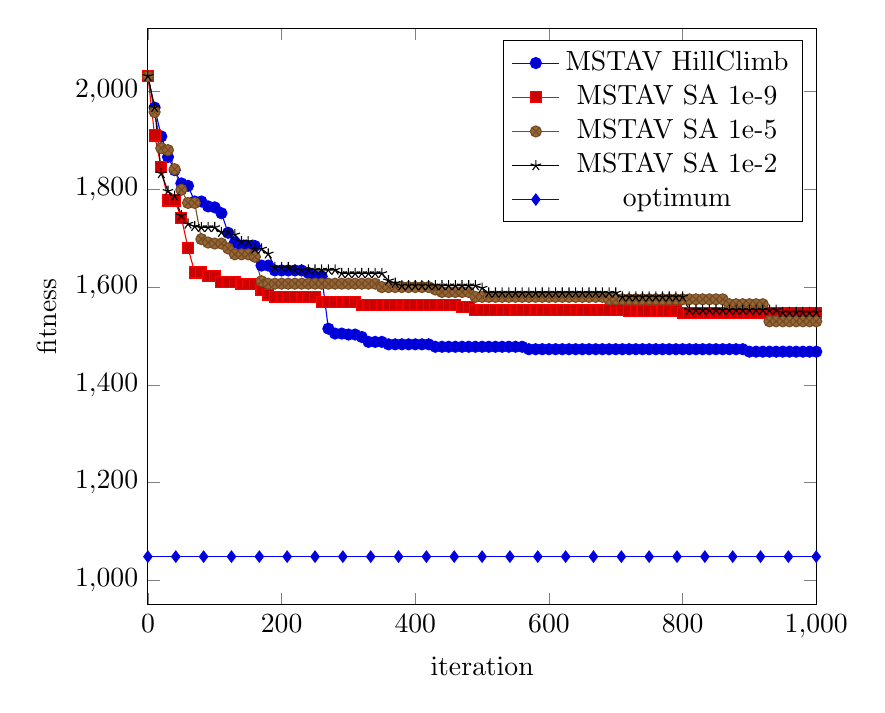
\begin{tikzpicture}
 \begin{axis}[
   width=0.7\textwidth,
   scale only axis,
   xlabel=iteration,
   ylabel=fitness,
   xmin=0,xmax=1000,
   domain=0:1000]
   \addplot coordinates {
     (0,2031)
     (10,1967)
     (20,1908)
     (30,1866)
     (40,1839)
     (50,1812)
     (60,1807)
     (70,1775)
     (80,1775)
     (90,1765)
     (100,1763)
     (110,1751)
     (120,1711)
     (130,1691)
     (140,1684)
     (150,1684)
     (160,1684)
     (170,1644)
     (180,1644)
     (190,1634)
     (200,1634)
     (210,1634)
     (220,1634)
     (230,1634)
     (240,1629)
     (250,1622)
     (260,1622)
     (270,1515)
     (280,1505)
     (290,1505)
     (300,1503)
     (310,1503)
     (320,1498)
     (330,1488)
     (340,1488)
     (350,1488)
     (360,1483)
     (370,1483)
     (380,1483)
     (390,1483)
     (400,1483)
     (410,1483)
     (420,1483)
     (430,1478)
     (440,1478)
     (450,1478)
     (460,1478)
     (470,1478)
     (480,1478)
     (490,1478)
     (500,1478)
     (510,1478)
     (520,1478)
     (530,1478)
     (540,1478)
     (550,1478)
     (560,1478)
     (570,1473)
     (580,1473)
     (590,1473)
     (600,1473)
     (610,1473)
     (620,1473)
     (630,1473)
     (640,1473)
     (650,1473)
     (660,1473)
     (670,1473)
     (680,1473)
     (690,1473)
     (700,1473)
     (710,1473)
     (720,1473)
     (730,1473)
     (740,1473)
     (750,1473)
     (760,1473)
     (770,1473)
     (780,1473)
     (790,1473)
     (800,1473)
     (810,1473)
     (820,1473)
     (830,1473)
     (840,1473)
     (850,1473)
     (860,1473)
     (870,1473)
     (880,1473)
     (890,1473)
     (900,1468)
     (910,1468)
     (920,1468)
     (930,1468)
     (940,1468)
     (950,1468)
     (960,1468)
     (970,1468)
     (980,1468)
     (990,1468)
     (1000,1468)
   };
   \addlegendentry{MSTAV HillClimb}
   \addplot coordinates {
     (0,2031)
     (10,1910)
     (20,1845)
     (30,1777)
     (40,1777)
     (50,1742)
     (60,1680)
     (70,1630)
     (80,1630)
     (90,1623)
     (100,1623)
     (110,1611)
     (120,1611)
     (130,1611)
     (140,1606)
     (150,1606)
     (160,1606)
     (170,1594)
     (180,1584)
     (190,1579)
     (200,1579)
     (210,1579)
     (220,1579)
     (230,1579)
     (240,1579)
     (250,1579)
     (260,1569)
     (270,1569)
     (280,1569)
     (290,1569)
     (300,1569)
     (310,1569)
     (320,1564)
     (330,1564)
     (340,1564)
     (350,1564)
     (360,1564)
     (370,1564)
     (380,1564)
     (390,1564)
     (400,1564)
     (410,1564)
     (420,1564)
     (430,1564)
     (440,1564)
     (450,1564)
     (460,1564)
     (470,1559)
     (480,1559)
     (490,1554)
     (500,1554)
     (510,1554)
     (520,1554)
     (530,1554)
     (540,1554)
     (550,1554)
     (560,1554)
     (570,1554)
     (580,1554)
     (590,1554)
     (600,1554)
     (610,1554)
     (620,1554)
     (630,1554)
     (640,1554)
     (650,1554)
     (660,1554)
     (670,1554)
     (680,1554)
     (690,1554)
     (700,1554)
     (710,1554)
     (720,1552)
     (730,1552)
     (740,1552)
     (750,1552)
     (760,1552)
     (770,1552)
     (780,1552)
     (790,1552)
     (800,1547)
     (810,1547)
     (820,1547)
     (830,1547)
     (840,1547)
     (850,1547)
     (860,1547)
     (870,1547)
     (880,1547)
     (890,1547)
     (900,1547)
     (910,1547)
     (920,1547)
     (930,1547)
     (940,1547)
     (950,1547)
     (960,1547)
     (970,1547)
     (980,1547)
     (990,1547)
     (1000,1547)
   };
   \addlegendentry{MSTAV SA 1e-9}
   \addplot coordinates {
     (0,2031)
     (10,1958)
     (20,1884)
     (30,1880)
     (40,1841)
     (50,1799)
     (60,1772)
     (70,1772)
     (80,1698)
     (90,1691)
     (100,1689)
     (110,1689)
     (120,1679)
     (130,1667)
     (140,1667)
     (150,1667)
     (160,1662)
     (170,1612)
     (180,1607)
     (190,1607)
     (200,1607)
     (210,1607)
     (220,1607)
     (230,1607)
     (240,1607)
     (250,1607)
     (260,1607)
     (270,1607)
     (280,1607)
     (290,1607)
     (300,1607)
     (310,1607)
     (320,1607)
     (330,1607)
     (340,1607)
     (350,1600)
     (360,1600)
     (370,1600)
     (380,1600)
     (390,1600)
     (400,1600)
     (410,1600)
     (420,1600)
     (430,1595)
     (440,1590)
     (450,1590)
     (460,1590)
     (470,1590)
     (480,1590)
     (490,1580)
     (500,1580)
     (510,1580)
     (520,1580)
     (530,1580)
     (540,1580)
     (550,1580)
     (560,1580)
     (570,1580)
     (580,1580)
     (590,1580)
     (600,1580)
     (610,1580)
     (620,1580)
     (630,1580)
     (640,1580)
     (650,1580)
     (660,1580)
     (670,1580)
     (680,1580)
     (690,1575)
     (700,1575)
     (710,1575)
     (720,1575)
     (730,1575)
     (740,1575)
     (750,1575)
     (760,1575)
     (770,1575)
     (780,1575)
     (790,1575)
     (800,1575)
     (810,1575)
     (820,1575)
     (830,1575)
     (840,1575)
     (850,1575)
     (860,1575)
     (870,1565)
     (880,1565)
     (890,1565)
     (900,1565)
     (910,1565)
     (920,1565)
     (930,1530)
     (940,1530)
     (950,1530)
     (960,1530)
     (970,1530)
     (980,1530)
     (990,1530)
     (1000,1530)
   };
   \addlegendentry{MSTAV SA 1e-5}
   \addplot coordinates {
     (0,2031)
     (10,1967)
     (20,1832)
     (30,1796)
     (40,1786)
     (50,1746)
     (60,1729)
     (70,1724)
     (80,1722)
     (90,1722)
     (100,1722)
     (110,1712)
     (120,1712)
     (130,1707)
     (140,1693)
     (150,1693)
     (160,1678)
     (170,1678)
     (180,1668)
     (190,1640)
     (200,1640)
     (210,1640)
     (220,1635)
     (230,1635)
     (240,1635)
     (250,1635)
     (260,1635)
     (270,1635)
     (280,1635)
     (290,1628)
     (300,1628)
     (310,1628)
     (320,1628)
     (330,1628)
     (340,1628)
     (350,1628)
     (360,1613)
     (370,1608)
     (380,1603)
     (390,1603)
     (400,1603)
     (410,1603)
     (420,1603)
     (430,1603)
     (440,1603)
     (450,1603)
     (460,1603)
     (470,1603)
     (480,1603)
     (490,1603)
     (500,1598)
     (510,1588)
     (520,1588)
     (530,1588)
     (540,1588)
     (550,1588)
     (560,1588)
     (570,1588)
     (580,1588)
     (590,1588)
     (600,1588)
     (610,1588)
     (620,1588)
     (630,1588)
     (640,1588)
     (650,1588)
     (660,1588)
     (670,1588)
     (680,1588)
     (690,1588)
     (700,1588)
     (710,1580)
     (720,1580)
     (730,1580)
     (740,1580)
     (750,1580)
     (760,1580)
     (770,1580)
     (780,1580)
     (790,1580)
     (800,1580)
     (810,1553)
     (820,1553)
     (830,1553)
     (840,1553)
     (850,1553)
     (860,1553)
     (870,1553)
     (880,1553)
     (890,1553)
     (900,1553)
     (910,1553)
     (920,1553)
     (930,1553)
     (940,1553)
     (950,1548)
     (960,1548)
     (970,1548)
     (980,1548)
     (990,1548)
     (1000,1548)
   };
   \addlegendentry{MSTAV SA 1e-2}
   \addplot {1049.000000};
   \addlegendentry{optimum}
 \end{axis}
 \end{tikzpicture}

\end{figure}
\begin{figure}[H]
\pgfsetplotmarksize{0pt}
 \centering
 \caption{\label{MSTAV-berlin52}MSTAV-berlin52},
 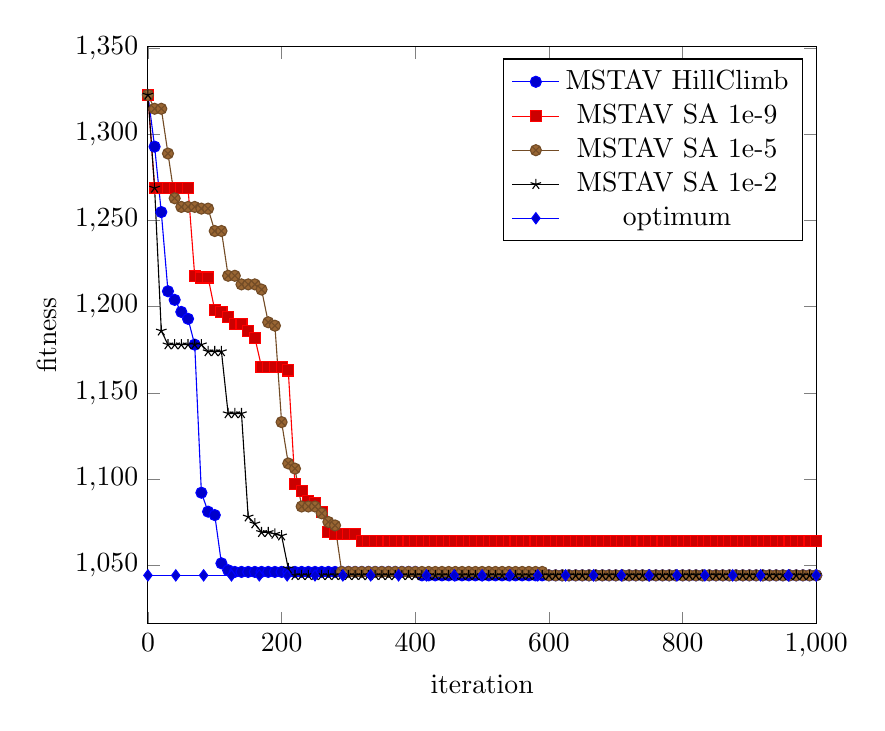
\begin{tikzpicture}
 \begin{axis}[
   width=0.7\textwidth,
   scale only axis,
   xlabel=iteration,
   ylabel=fitness,
   xmin=0,xmax=1000,
   domain=0:1000]
   \addplot coordinates {
     (0,1323)
     (10,1293)
     (20,1255)
     (30,1209)
     (40,1204)
     (50,1197)
     (60,1193)
     (70,1178)
     (80,1092)
     (90,1081)
     (100,1079)
     (110,1051)
     (120,1047)
     (130,1046)
     (140,1046)
     (150,1046)
     (160,1046)
     (170,1046)
     (180,1046)
     (190,1046)
     (200,1046)
     (210,1046)
     (220,1046)
     (230,1046)
     (240,1046)
     (250,1046)
     (260,1046)
     (270,1046)
     (280,1046)
     (290,1046)
     (300,1046)
     (310,1046)
     (320,1046)
     (330,1046)
     (340,1046)
     (350,1046)
     (360,1046)
     (370,1046)
     (380,1046)
     (390,1046)
     (400,1046)
     (410,1044)
     (420,1044)
     (430,1044)
     (440,1044)
     (450,1044)
     (460,1044)
     (470,1044)
     (480,1044)
     (490,1044)
     (500,1044)
     (510,1044)
     (520,1044)
     (530,1044)
     (540,1044)
     (550,1044)
     (560,1044)
     (570,1044)
     (580,1044)
     (590,1044)
     (600,1044)
     (610,1044)
     (620,1044)
     (630,1044)
     (640,1044)
     (650,1044)
     (660,1044)
     (670,1044)
     (680,1044)
     (690,1044)
     (700,1044)
     (710,1044)
     (720,1044)
     (730,1044)
     (740,1044)
     (750,1044)
     (760,1044)
     (770,1044)
     (780,1044)
     (790,1044)
     (800,1044)
     (810,1044)
     (820,1044)
     (830,1044)
     (840,1044)
     (850,1044)
     (860,1044)
     (870,1044)
     (880,1044)
     (890,1044)
     (900,1044)
     (910,1044)
     (920,1044)
     (930,1044)
     (940,1044)
     (950,1044)
     (960,1044)
     (970,1044)
     (980,1044)
     (990,1044)
     (1000,1044)
   };
   \addlegendentry{MSTAV HillClimb}
   \addplot coordinates {
     (0,1323)
     (10,1269)
     (20,1269)
     (30,1269)
     (40,1269)
     (50,1269)
     (60,1269)
     (70,1218)
     (80,1217)
     (90,1217)
     (100,1198)
     (110,1197)
     (120,1194)
     (130,1190)
     (140,1190)
     (150,1186)
     (160,1182)
     (170,1165)
     (180,1165)
     (190,1165)
     (200,1165)
     (210,1163)
     (220,1097)
     (230,1093)
     (240,1087)
     (250,1086)
     (260,1081)
     (270,1069)
     (280,1068)
     (290,1068)
     (300,1068)
     (310,1068)
     (320,1064)
     (330,1064)
     (340,1064)
     (350,1064)
     (360,1064)
     (370,1064)
     (380,1064)
     (390,1064)
     (400,1064)
     (410,1064)
     (420,1064)
     (430,1064)
     (440,1064)
     (450,1064)
     (460,1064)
     (470,1064)
     (480,1064)
     (490,1064)
     (500,1064)
     (510,1064)
     (520,1064)
     (530,1064)
     (540,1064)
     (550,1064)
     (560,1064)
     (570,1064)
     (580,1064)
     (590,1064)
     (600,1064)
     (610,1064)
     (620,1064)
     (630,1064)
     (640,1064)
     (650,1064)
     (660,1064)
     (670,1064)
     (680,1064)
     (690,1064)
     (700,1064)
     (710,1064)
     (720,1064)
     (730,1064)
     (740,1064)
     (750,1064)
     (760,1064)
     (770,1064)
     (780,1064)
     (790,1064)
     (800,1064)
     (810,1064)
     (820,1064)
     (830,1064)
     (840,1064)
     (850,1064)
     (860,1064)
     (870,1064)
     (880,1064)
     (890,1064)
     (900,1064)
     (910,1064)
     (920,1064)
     (930,1064)
     (940,1064)
     (950,1064)
     (960,1064)
     (970,1064)
     (980,1064)
     (990,1064)
     (1000,1064)
   };
   \addlegendentry{MSTAV SA 1e-9}
   \addplot coordinates {
     (0,1323)
     (10,1315)
     (20,1315)
     (30,1289)
     (40,1263)
     (50,1258)
     (60,1258)
     (70,1258)
     (80,1257)
     (90,1257)
     (100,1244)
     (110,1244)
     (120,1218)
     (130,1218)
     (140,1213)
     (150,1213)
     (160,1213)
     (170,1210)
     (180,1191)
     (190,1189)
     (200,1133)
     (210,1109)
     (220,1106)
     (230,1084)
     (240,1084)
     (250,1084)
     (260,1080)
     (270,1075)
     (280,1073)
     (290,1046)
     (300,1046)
     (310,1046)
     (320,1046)
     (330,1046)
     (340,1046)
     (350,1046)
     (360,1046)
     (370,1046)
     (380,1046)
     (390,1046)
     (400,1046)
     (410,1046)
     (420,1046)
     (430,1046)
     (440,1046)
     (450,1046)
     (460,1046)
     (470,1046)
     (480,1046)
     (490,1046)
     (500,1046)
     (510,1046)
     (520,1046)
     (530,1046)
     (540,1046)
     (550,1046)
     (560,1046)
     (570,1046)
     (580,1046)
     (590,1046)
     (600,1044)
     (610,1044)
     (620,1044)
     (630,1044)
     (640,1044)
     (650,1044)
     (660,1044)
     (670,1044)
     (680,1044)
     (690,1044)
     (700,1044)
     (710,1044)
     (720,1044)
     (730,1044)
     (740,1044)
     (750,1044)
     (760,1044)
     (770,1044)
     (780,1044)
     (790,1044)
     (800,1044)
     (810,1044)
     (820,1044)
     (830,1044)
     (840,1044)
     (850,1044)
     (860,1044)
     (870,1044)
     (880,1044)
     (890,1044)
     (900,1044)
     (910,1044)
     (920,1044)
     (930,1044)
     (940,1044)
     (950,1044)
     (960,1044)
     (970,1044)
     (980,1044)
     (990,1044)
     (1000,1044)
   };
   \addlegendentry{MSTAV SA 1e-5}
   \addplot coordinates {
     (0,1323)
     (10,1269)
     (20,1186)
     (30,1178)
     (40,1178)
     (50,1178)
     (60,1178)
     (70,1178)
     (80,1178)
     (90,1174)
     (100,1174)
     (110,1174)
     (120,1138)
     (130,1138)
     (140,1138)
     (150,1078)
     (160,1074)
     (170,1069)
     (180,1069)
     (190,1068)
     (200,1067)
     (210,1048)
     (220,1044)
     (230,1044)
     (240,1044)
     (250,1044)
     (260,1044)
     (270,1044)
     (280,1044)
     (290,1044)
     (300,1044)
     (310,1044)
     (320,1044)
     (330,1044)
     (340,1044)
     (350,1044)
     (360,1044)
     (370,1044)
     (380,1044)
     (390,1044)
     (400,1044)
     (410,1044)
     (420,1044)
     (430,1044)
     (440,1044)
     (450,1044)
     (460,1044)
     (470,1044)
     (480,1044)
     (490,1044)
     (500,1044)
     (510,1044)
     (520,1044)
     (530,1044)
     (540,1044)
     (550,1044)
     (560,1044)
     (570,1044)
     (580,1044)
     (590,1044)
     (600,1044)
     (610,1044)
     (620,1044)
     (630,1044)
     (640,1044)
     (650,1044)
     (660,1044)
     (670,1044)
     (680,1044)
     (690,1044)
     (700,1044)
     (710,1044)
     (720,1044)
     (730,1044)
     (740,1044)
     (750,1044)
     (760,1044)
     (770,1044)
     (780,1044)
     (790,1044)
     (800,1044)
     (810,1044)
     (820,1044)
     (830,1044)
     (840,1044)
     (850,1044)
     (860,1044)
     (870,1044)
     (880,1044)
     (890,1044)
     (900,1044)
     (910,1044)
     (920,1044)
     (930,1044)
     (940,1044)
     (950,1044)
     (960,1044)
     (970,1044)
     (980,1044)
     (990,1044)
     (1000,1044)
   };
   \addlegendentry{MSTAV SA 1e-2}
   \addplot {1044.000000};
   \addlegendentry{optimum}
 \end{axis}
 \end{tikzpicture}

\end{figure}

\subsection{CBC and MSTAV convergence comparison}
TODO: napisac, ze MSTAV > CRC, zasugerowac dlaczego

\begin{figure}[H]
\pgfsetplotmarksize{0pt}
\begin{figure}
 \centering
 \caption{\label{CBCvsMSTAV-01sEV100K30}CBCvsMSTAV-01sEV100K30},
 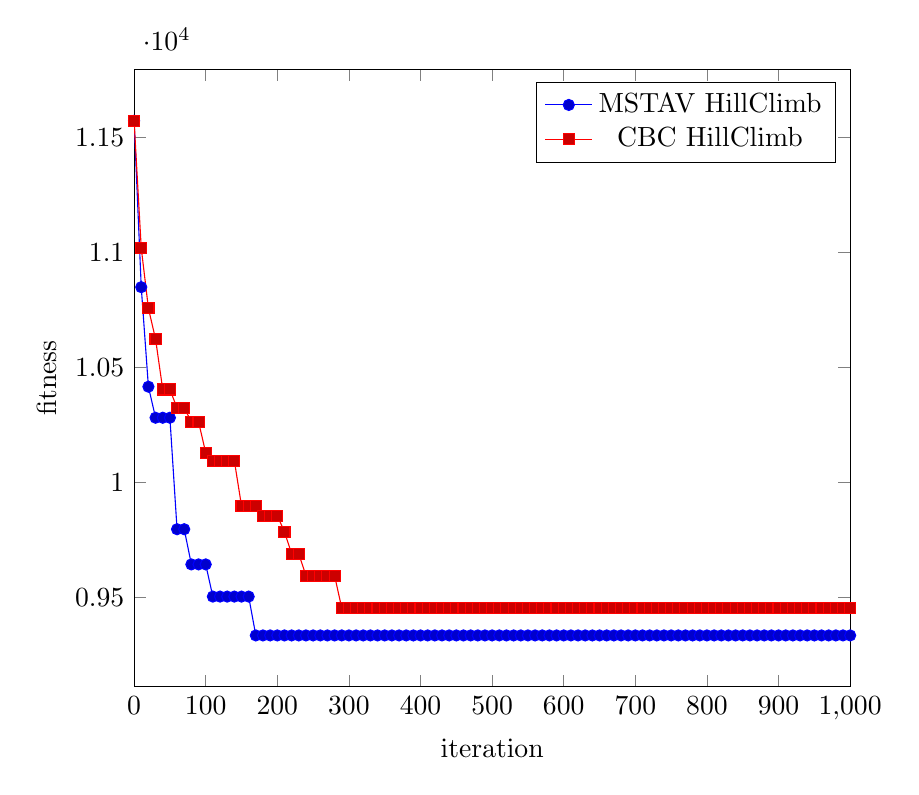
\begin{tikzpicture}
 \begin{axis}[
   width=0.75\textwidth,
   scale only axis,
   xlabel=iteration,
   ylabel=fitness,
   xmin=0,xmax=1000,
   domain=0:1000]
   \addplot coordinates {
     (0,11574)
     (10,10850)
     (20,10417)
     (30,10282)
     (40,10282)
     (50,10282)
     (60,9797)
     (70,9797)
     (80,9644)
     (90,9644)
     (100,9644)
     (110,9504)
     (120,9504)
     (130,9504)
     (140,9504)
     (150,9504)
     (160,9504)
     (170,9335)
     (180,9335)
     (190,9335)
     (200,9335)
     (210,9335)
     (220,9335)
     (230,9335)
     (240,9335)
     (250,9335)
     (260,9335)
     (270,9335)
     (280,9335)
     (290,9335)
     (300,9335)
     (310,9335)
     (320,9335)
     (330,9335)
     (340,9335)
     (350,9335)
     (360,9335)
     (370,9335)
     (380,9335)
     (390,9335)
     (400,9335)
     (410,9335)
     (420,9335)
     (430,9335)
     (440,9335)
     (450,9335)
     (460,9335)
     (470,9335)
     (480,9335)
     (490,9335)
     (500,9335)
     (510,9335)
     (520,9335)
     (530,9335)
     (540,9335)
     (550,9335)
     (560,9335)
     (570,9335)
     (580,9335)
     (590,9335)
     (600,9335)
     (610,9335)
     (620,9335)
     (630,9335)
     (640,9335)
     (650,9335)
     (660,9335)
     (670,9335)
     (680,9335)
     (690,9335)
     (700,9335)
     (710,9335)
     (720,9335)
     (730,9335)
     (740,9335)
     (750,9335)
     (760,9335)
     (770,9335)
     (780,9335)
     (790,9335)
     (800,9335)
     (810,9335)
     (820,9335)
     (830,9335)
     (840,9335)
     (850,9335)
     (860,9335)
     (870,9335)
     (880,9335)
     (890,9335)
     (900,9335)
     (910,9335)
     (920,9335)
     (930,9335)
     (940,9335)
     (950,9335)
     (960,9335)
     (970,9335)
     (980,9335)
     (990,9335)
     (1000,9335)
   };
   \addlegendentry{MSTAV HillClimb}
   \addplot coordinates {
     (0,11574)
     (10,11020)
     (20,10758)
     (30,10624)
     (40,10405)
     (50,10405)
     (60,10324)
     (70,10324)
     (80,10265)
     (90,10265)
     (100,10130)
     (110,10095)
     (120,10095)
     (130,10095)
     (140,10095)
     (150,9899)
     (160,9899)
     (170,9899)
     (180,9856)
     (190,9856)
     (200,9856)
     (210,9786)
     (220,9690)
     (230,9690)
     (240,9595)
     (250,9595)
     (260,9595)
     (270,9595)
     (280,9595)
     (290,9454)
     (300,9454)
     (310,9454)
     (320,9454)
     (330,9454)
     (340,9454)
     (350,9454)
     (360,9454)
     (370,9454)
     (380,9454)
     (390,9454)
     (400,9454)
     (410,9454)
     (420,9454)
     (430,9454)
     (440,9454)
     (450,9454)
     (460,9454)
     (470,9454)
     (480,9454)
     (490,9454)
     (500,9454)
     (510,9454)
     (520,9454)
     (530,9454)
     (540,9454)
     (550,9454)
     (560,9454)
     (570,9454)
     (580,9454)
     (590,9454)
     (600,9454)
     (610,9454)
     (620,9454)
     (630,9454)
     (640,9454)
     (650,9454)
     (660,9454)
     (670,9454)
     (680,9454)
     (690,9454)
     (700,9454)
     (710,9454)
     (720,9454)
     (730,9454)
     (740,9454)
     (750,9454)
     (760,9454)
     (770,9454)
     (780,9454)
     (790,9454)
     (800,9454)
     (810,9454)
     (820,9454)
     (830,9454)
     (840,9454)
     (850,9454)
     (860,9454)
     (870,9454)
     (880,9454)
     (890,9454)
     (900,9454)
     (910,9454)
     (920,9454)
     (930,9454)
     (940,9454)
     (950,9454)
     (960,9454)
     (970,9454)
     (980,9454)
     (990,9454)
     (1000,9454)
   };
   \addlegendentry{CBC HillClimb}
 \end{axis}
 \end{tikzpicture}
\end{figure}

\end{figure}
\begin{figure}[H]
\pgfsetplotmarksize{0pt}
\begin{figure}
 \centering
 \caption{\label{CBCvsMSTAV-01sRV1000K150}CBCvsMSTAV-01sRV1000K150},
 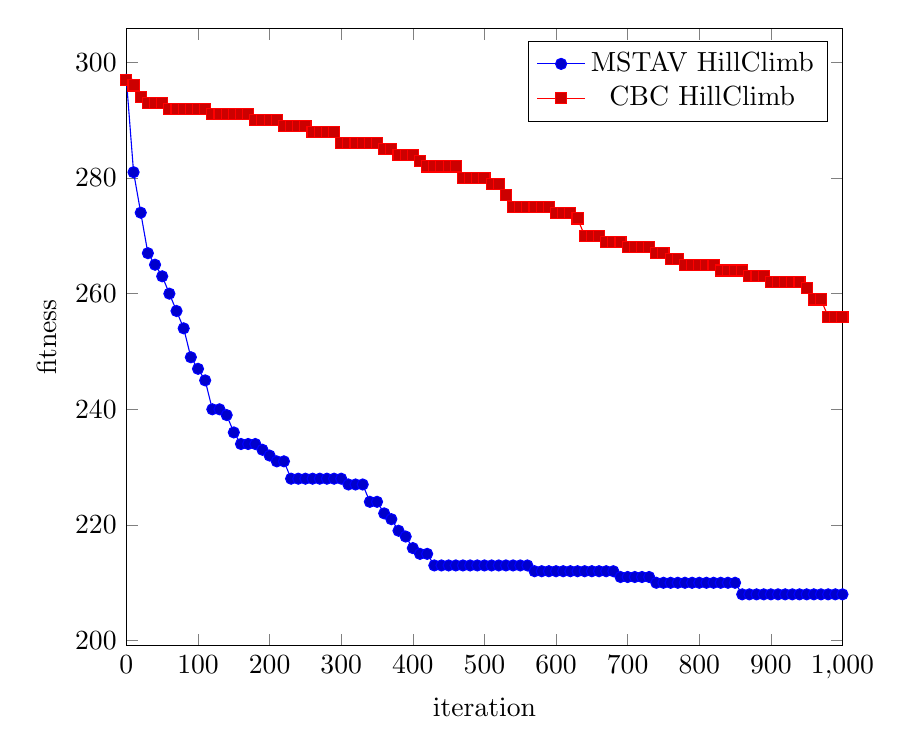
\begin{tikzpicture}
 \begin{axis}[
   width=0.75\textwidth,
   scale only axis,
   xlabel=iteration,
   ylabel=fitness,
   xmin=0,xmax=1000,
   domain=0:1000]
   \addplot coordinates {
     (0,297)
     (10,281)
     (20,274)
     (30,267)
     (40,265)
     (50,263)
     (60,260)
     (70,257)
     (80,254)
     (90,249)
     (100,247)
     (110,245)
     (120,240)
     (130,240)
     (140,239)
     (150,236)
     (160,234)
     (170,234)
     (180,234)
     (190,233)
     (200,232)
     (210,231)
     (220,231)
     (230,228)
     (240,228)
     (250,228)
     (260,228)
     (270,228)
     (280,228)
     (290,228)
     (300,228)
     (310,227)
     (320,227)
     (330,227)
     (340,224)
     (350,224)
     (360,222)
     (370,221)
     (380,219)
     (390,218)
     (400,216)
     (410,215)
     (420,215)
     (430,213)
     (440,213)
     (450,213)
     (460,213)
     (470,213)
     (480,213)
     (490,213)
     (500,213)
     (510,213)
     (520,213)
     (530,213)
     (540,213)
     (550,213)
     (560,213)
     (570,212)
     (580,212)
     (590,212)
     (600,212)
     (610,212)
     (620,212)
     (630,212)
     (640,212)
     (650,212)
     (660,212)
     (670,212)
     (680,212)
     (690,211)
     (700,211)
     (710,211)
     (720,211)
     (730,211)
     (740,210)
     (750,210)
     (760,210)
     (770,210)
     (780,210)
     (790,210)
     (800,210)
     (810,210)
     (820,210)
     (830,210)
     (840,210)
     (850,210)
     (860,208)
     (870,208)
     (880,208)
     (890,208)
     (900,208)
     (910,208)
     (920,208)
     (930,208)
     (940,208)
     (950,208)
     (960,208)
     (970,208)
     (980,208)
     (990,208)
     (1000,208)
   };
   \addlegendentry{MSTAV HillClimb}
   \addplot coordinates {
     (0,297)
     (10,296)
     (20,294)
     (30,293)
     (40,293)
     (50,293)
     (60,292)
     (70,292)
     (80,292)
     (90,292)
     (100,292)
     (110,292)
     (120,291)
     (130,291)
     (140,291)
     (150,291)
     (160,291)
     (170,291)
     (180,290)
     (190,290)
     (200,290)
     (210,290)
     (220,289)
     (230,289)
     (240,289)
     (250,289)
     (260,288)
     (270,288)
     (280,288)
     (290,288)
     (300,286)
     (310,286)
     (320,286)
     (330,286)
     (340,286)
     (350,286)
     (360,285)
     (370,285)
     (380,284)
     (390,284)
     (400,284)
     (410,283)
     (420,282)
     (430,282)
     (440,282)
     (450,282)
     (460,282)
     (470,280)
     (480,280)
     (490,280)
     (500,280)
     (510,279)
     (520,279)
     (530,277)
     (540,275)
     (550,275)
     (560,275)
     (570,275)
     (580,275)
     (590,275)
     (600,274)
     (610,274)
     (620,274)
     (630,273)
     (640,270)
     (650,270)
     (660,270)
     (670,269)
     (680,269)
     (690,269)
     (700,268)
     (710,268)
     (720,268)
     (730,268)
     (740,267)
     (750,267)
     (760,266)
     (770,266)
     (780,265)
     (790,265)
     (800,265)
     (810,265)
     (820,265)
     (830,264)
     (840,264)
     (850,264)
     (860,264)
     (870,263)
     (880,263)
     (890,263)
     (900,262)
     (910,262)
     (920,262)
     (930,262)
     (940,262)
     (950,261)
     (960,259)
     (970,259)
     (980,256)
     (990,256)
     (1000,256)
   };
   \addlegendentry{CBC HillClimb}
 \end{axis}
 \end{tikzpicture}
\end{figure}

\end{figure}
\begin{figure}[H]
\pgfsetplotmarksize{0pt}
\begin{figure}
 \centering
 \caption{\label{CBCvsMSTAV-d05}CBCvsMSTAV-d05},
 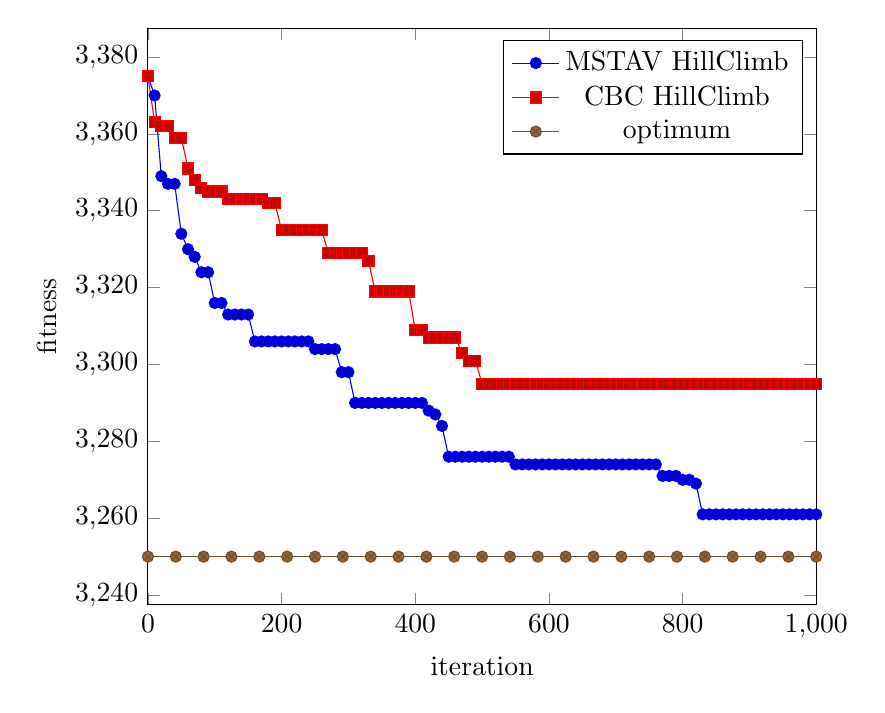
\begin{tikzpicture}
 \begin{axis}[
   width=0.7\textwidth,
   scale only axis,
   xlabel=iteration,
   ylabel=fitness,
   xmin=0,xmax=1000,
   domain=0:1000]
   \addplot coordinates {
     (0,3375)
     (10,3370)
     (20,3349)
     (30,3347)
     (40,3347)
     (50,3334)
     (60,3330)
     (70,3328)
     (80,3324)
     (90,3324)
     (100,3316)
     (110,3316)
     (120,3313)
     (130,3313)
     (140,3313)
     (150,3313)
     (160,3306)
     (170,3306)
     (180,3306)
     (190,3306)
     (200,3306)
     (210,3306)
     (220,3306)
     (230,3306)
     (240,3306)
     (250,3304)
     (260,3304)
     (270,3304)
     (280,3304)
     (290,3298)
     (300,3298)
     (310,3290)
     (320,3290)
     (330,3290)
     (340,3290)
     (350,3290)
     (360,3290)
     (370,3290)
     (380,3290)
     (390,3290)
     (400,3290)
     (410,3290)
     (420,3288)
     (430,3287)
     (440,3284)
     (450,3276)
     (460,3276)
     (470,3276)
     (480,3276)
     (490,3276)
     (500,3276)
     (510,3276)
     (520,3276)
     (530,3276)
     (540,3276)
     (550,3274)
     (560,3274)
     (570,3274)
     (580,3274)
     (590,3274)
     (600,3274)
     (610,3274)
     (620,3274)
     (630,3274)
     (640,3274)
     (650,3274)
     (660,3274)
     (670,3274)
     (680,3274)
     (690,3274)
     (700,3274)
     (710,3274)
     (720,3274)
     (730,3274)
     (740,3274)
     (750,3274)
     (760,3274)
     (770,3271)
     (780,3271)
     (790,3271)
     (800,3270)
     (810,3270)
     (820,3269)
     (830,3261)
     (840,3261)
     (850,3261)
     (860,3261)
     (870,3261)
     (880,3261)
     (890,3261)
     (900,3261)
     (910,3261)
     (920,3261)
     (930,3261)
     (940,3261)
     (950,3261)
     (960,3261)
     (970,3261)
     (980,3261)
     (990,3261)
     (1000,3261)
   };
   \addlegendentry{MSTAV HillClimb}
   \addplot coordinates {
     (0,3375)
     (10,3363)
     (20,3362)
     (30,3362)
     (40,3359)
     (50,3359)
     (60,3351)
     (70,3348)
     (80,3346)
     (90,3345)
     (100,3345)
     (110,3345)
     (120,3343)
     (130,3343)
     (140,3343)
     (150,3343)
     (160,3343)
     (170,3343)
     (180,3342)
     (190,3342)
     (200,3335)
     (210,3335)
     (220,3335)
     (230,3335)
     (240,3335)
     (250,3335)
     (260,3335)
     (270,3329)
     (280,3329)
     (290,3329)
     (300,3329)
     (310,3329)
     (320,3329)
     (330,3327)
     (340,3319)
     (350,3319)
     (360,3319)
     (370,3319)
     (380,3319)
     (390,3319)
     (400,3309)
     (410,3309)
     (420,3307)
     (430,3307)
     (440,3307)
     (450,3307)
     (460,3307)
     (470,3303)
     (480,3301)
     (490,3301)
     (500,3295)
     (510,3295)
     (520,3295)
     (530,3295)
     (540,3295)
     (550,3295)
     (560,3295)
     (570,3295)
     (580,3295)
     (590,3295)
     (600,3295)
     (610,3295)
     (620,3295)
     (630,3295)
     (640,3295)
     (650,3295)
     (660,3295)
     (670,3295)
     (680,3295)
     (690,3295)
     (700,3295)
     (710,3295)
     (720,3295)
     (730,3295)
     (740,3295)
     (750,3295)
     (760,3295)
     (770,3295)
     (780,3295)
     (790,3295)
     (800,3295)
     (810,3295)
     (820,3295)
     (830,3295)
     (840,3295)
     (850,3295)
     (860,3295)
     (870,3295)
     (880,3295)
     (890,3295)
     (900,3295)
     (910,3295)
     (920,3295)
     (930,3295)
     (940,3295)
     (950,3295)
     (960,3295)
     (970,3295)
     (980,3295)
     (990,3295)
     (1000,3295)
   };
   \addlegendentry{CBC HillClimb}
   \addplot {3250.000000};
   \addlegendentry{optimum}
 \end{axis}
 \end{tikzpicture}
\end{figure}

\end{figure}
\begin{figure}[H]
\pgfsetplotmarksize{0pt}
 \centering
 \caption{\label{CBCvsMSTAV-gap1307}CBCvsMSTAV-gap1307},
 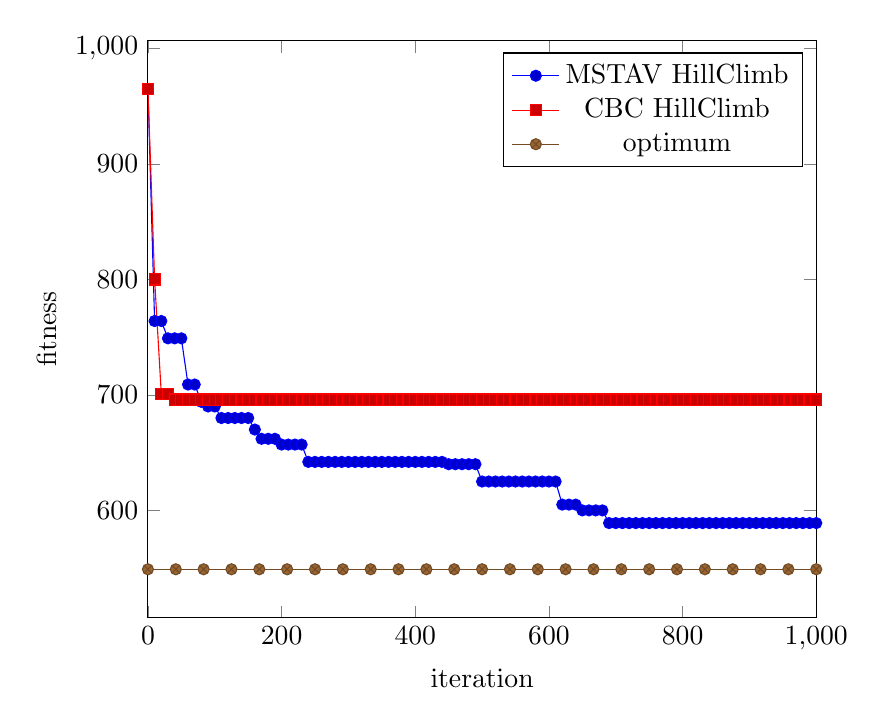
\begin{tikzpicture}
 \begin{axis}[
   width=0.7\textwidth,
   scale only axis,
   xlabel=iteration,
   ylabel=fitness,
   xmin=0,xmax=1000,
   domain=0:1000]
   \addplot coordinates {
     (0,965)
     (10,764)
     (20,764)
     (30,749)
     (40,749)
     (50,749)
     (60,709)
     (70,709)
     (80,694)
     (90,690)
     (100,690)
     (110,680)
     (120,680)
     (130,680)
     (140,680)
     (150,680)
     (160,670)
     (170,662)
     (180,662)
     (190,662)
     (200,657)
     (210,657)
     (220,657)
     (230,657)
     (240,642)
     (250,642)
     (260,642)
     (270,642)
     (280,642)
     (290,642)
     (300,642)
     (310,642)
     (320,642)
     (330,642)
     (340,642)
     (350,642)
     (360,642)
     (370,642)
     (380,642)
     (390,642)
     (400,642)
     (410,642)
     (420,642)
     (430,642)
     (440,642)
     (450,640)
     (460,640)
     (470,640)
     (480,640)
     (490,640)
     (500,625)
     (510,625)
     (520,625)
     (530,625)
     (540,625)
     (550,625)
     (560,625)
     (570,625)
     (580,625)
     (590,625)
     (600,625)
     (610,625)
     (620,605)
     (630,605)
     (640,605)
     (650,600)
     (660,600)
     (670,600)
     (680,600)
     (690,589)
     (700,589)
     (710,589)
     (720,589)
     (730,589)
     (740,589)
     (750,589)
     (760,589)
     (770,589)
     (780,589)
     (790,589)
     (800,589)
     (810,589)
     (820,589)
     (830,589)
     (840,589)
     (850,589)
     (860,589)
     (870,589)
     (880,589)
     (890,589)
     (900,589)
     (910,589)
     (920,589)
     (930,589)
     (940,589)
     (950,589)
     (960,589)
     (970,589)
     (980,589)
     (990,589)
     (1000,589)
   };
   \addlegendentry{MSTAV HillClimb}
   \addplot coordinates {
     (0,965)
     (10,800)
     (20,701)
     (30,701)
     (40,696)
     (50,696)
     (60,696)
     (70,696)
     (80,696)
     (90,696)
     (100,696)
     (110,696)
     (120,696)
     (130,696)
     (140,696)
     (150,696)
     (160,696)
     (170,696)
     (180,696)
     (190,696)
     (200,696)
     (210,696)
     (220,696)
     (230,696)
     (240,696)
     (250,696)
     (260,696)
     (270,696)
     (280,696)
     (290,696)
     (300,696)
     (310,696)
     (320,696)
     (330,696)
     (340,696)
     (350,696)
     (360,696)
     (370,696)
     (380,696)
     (390,696)
     (400,696)
     (410,696)
     (420,696)
     (430,696)
     (440,696)
     (450,696)
     (460,696)
     (470,696)
     (480,696)
     (490,696)
     (500,696)
     (510,696)
     (520,696)
     (530,696)
     (540,696)
     (550,696)
     (560,696)
     (570,696)
     (580,696)
     (590,696)
     (600,696)
     (610,696)
     (620,696)
     (630,696)
     (640,696)
     (650,696)
     (660,696)
     (670,696)
     (680,696)
     (690,696)
     (700,696)
     (710,696)
     (720,696)
     (730,696)
     (740,696)
     (750,696)
     (760,696)
     (770,696)
     (780,696)
     (790,696)
     (800,696)
     (810,696)
     (820,696)
     (830,696)
     (840,696)
     (850,696)
     (860,696)
     (870,696)
     (880,696)
     (890,696)
     (900,696)
     (910,696)
     (920,696)
     (930,696)
     (940,696)
     (950,696)
     (960,696)
     (970,696)
     (980,696)
     (990,696)
     (1000,696)
   };
   \addlegendentry{CBC HillClimb}
   \addplot {549.000000};
   \addlegendentry{optimum}
 \end{axis}
 \end{tikzpicture}

\end{figure}

\subsection{Comparison of found solutions' fitness}
After testing presented algorithms we have made following observations:
\begin{itemize}
\item fitness of solutions found by 2-approximation algorithm is almost always less than 1.1 times optimum,
\item local searches performed well on problem instances with less than thousand of vertices,
\item MSTAV gives better results than CBC most of the time,
\item MSTAV often finds better solutions than 2-approximation algorithm for problem instances with less than thousand of vertices,
\item for graphs with thousands of vertices 2-approximation algorithm finds much better solutions than local seaches.
\end{itemize}

\begin{figure}[H]
  \centering
  \begin{tabular}[ht]{|l||c|c|c|c|H}
\cline{1-5}
 & 01dEV100K20 & 01sEV1000K150 & 01sEV100K20 & 01dRV100K20 & \\ \cline{1-5}\cline{1-5} 
2-Approximation &3476 & 20605 & 5927 & 24 & \\ \cline{1-5}
MSTAV HillClimb &3376 & 20231 & 5785 & 22 & \\ \cline{1-5}
CBC HillClimb &3654 & 24213 & 6021 & 24 & \\ \cline{1-5}
\end{tabular}
  \caption{Results for sample of SFP tests for graphs with less than thousand vertices}
\end{figure}

\begin{figure}[H]
  \centering
  \begin{tabular}[ht]{|l||c|c|c|c|c|c|H}
\cline{1-7}
 & alut2764 & b13 & berlin52 & diw0250 & msm3277 & d15 & \\ \cline{1-7}\cline{1-7} 
Optimum &640 & 165 & 1044 & 350 & 869 & 1116 & \\ \cline{1-7}
2-Approximation &710 & 187 & 1078 & 363 & 912 & 1161 & \\ \cline{1-7}
MSTAV HillClimb &662 & 170 & 1044 & 467 & 1089 & 1126 & \\ \cline{1-7}
CBC HillClimb &1044 & 177 & 1103 & 518 & 1222 & 1186 & \\ \cline{1-7}
\end{tabular}
  \caption{Results for sample of STP tests for graphs with less than thousand vertices}
\end{figure}

\begin{figure}[H]
  \centering
  \begin{tabular}[ht]{|l||c|c|c|c|H}
\cline{1-5}
 & 04sEV1000K250 & 03sEV1000K150 & 01sRV1000K150 & 01sRV1000K250 & \\ \cline{1-5}\cline{1-5} 
2-Approximation &29569 & 17175 & 208 & 262 & \\ \cline{1-5}
MSTAV HillClimb &29624 & 17163 & 196 & 279 & \\ \cline{1-5}
CBC HillClimb &35091 & 21899 & 259 & 365 & \\ \cline{1-5}
\end{tabular}
  \caption{Results for sample of SFP tests for graphs with at least thousand of vertices}
\end{figure}

\begin{figure}[H]
  \centering
  \begin{tabular}[ht]{|l||c|c|c|c|c|c|H}
\cline{1-7}
 & alue2087 & d11 & diw0445 & e02 & taq0431 & msm3277 & \\ \cline{1-7}\cline{1-7} 
Optimum &1049 & 29 & 1363 & 214 & 897 & 869 & \\ \cline{1-7}
2-Approximation &1122 & 33 & 1453 & 255 & 980 & 912 & \\ \cline{1-7}
MSTAV HillClimb &1375 & 36 & 1827 & 361 & 1484 & 1233 & \\ \cline{1-7}
CBC HillClimb &1698 & 49 & 2321 & 442 & 1519 & 1263 & \\ \cline{1-7}
\end{tabular}
  \caption{Results for sample of STP tests for graphs with at least thousand of vertices}
\end{figure}

